\documentclass[12pt]{article}
\usepackage[utf8]{inputenc}
\usepackage{geometry}
\usepackage[T1]{fontenc}
\usepackage{amsfonts}
\usepackage{afterpage}
\usepackage{graphicx}
\usepackage{float}
\usepackage{url}
\usepackage{hyperref}
\usepackage{bookmark}
\usepackage[sorting=none]{biblatex}
\usepackage{multirow}
\usepackage[table,xcdraw]{xcolor}
\usepackage{pgf}
\usepackage{xurl}
\usepackage{tabularray}
\usepackage{tabulary}
\usepackage{fancyhdr}
\usepackage[maxfloats=30,morefloats=12]{morefloats}
\usepackage{multicol}
\usepackage[dvipsnames]{xcolor}
\usepackage{awesomebox}
\usepackage{subcaption}
\usepackage{awesomebox}
\usepackage{pgfornament}
\usepackage[export]{adjustbox}
\usepackage{biblatex} %Imports biblatex package
\usepackage{tikzlings}

\addbibresource{howto.bib} %Import the bibliography file
\fontfamily{put}\selectfont
\setlength{\columnsep}{40pt}
\setlength{\voffset}{0.5cm}
\setlength{\headsep}{40pt}
\setlength{\headheight}{34.06914pt} % Fix for fancyhdr error
\addtolength{\topmargin}{-22.06914pt} % Adjusted top margin as suggested by fancyhdr
\geometry{legalpaper, portrait, margin=2.3cm}

% Header and footer
\pagestyle{fancy}
\fancyhead[C]{
\includegraphics[width=0.05\textwidth]{images/escudo.png}}
\fancyhead[L]{\textbf{Tópicos II}\\ Universidad de Concepción}
\fancyhead[R]{\textbf{Florencia Fuentes}\\flofuentes2021@udec.cl}
\fancyfoot{}
% for adjust width environment
\usepackage[strict]{changepage}

% for formal definitions
\usepackage{framed}

%\definecolor{formalshade}{rgb}{0.95,0.95,1}
\definecolor{formalshade}{rgb}{.97, .88, .94}

\newenvironment{formal}{
  \def\FrameCommand{
    \hspace{1pt}
    {\color{White}\vrule width 2pt}
    {\color{Lavender}\vrule width 4pt}
    \colorbox{formalshade!40!white}
  }
  \MakeFramed{\advance\hsize-\width\FrameRestore}%
  \noindent\hspace{-4.55pt}% disable indenting first paragraph
  \begin{adjustwidth}{}{7pt}%
  \vspace{2pt}\vspace{2pt}
}
{\vspace{2pt}\end{adjustwidth}\endMakeFramed}

\renewcommand{\headrulewidth}{0.1pt}

\usepackage{tikz}

\usepackage{tcolorbox}
\tcbuselibrary{minted}
\newtcblisting{mybox}{colback=white,minted language=latex,listing side text,righthand width=.5\textwidth}
\usetikzlibrary{ducks}
\usepackage{tikzducks}

\definecolor{titlepagecolor}{cmyk}{0,.49,.15,.11}

\newcommand\titlepagedecoration{%
\begin{tikzpicture}[remember picture,overlay,shorten >= -10pt]

\coordinate (aux1) at ([yshift=-15pt]current page.north east);
\coordinate (aux2) at ([yshift=-410pt]current page.north east);
\coordinate (aux3) at ([xshift=-4.5cm]current page.north east);
\coordinate (aux4) at ([yshift=-150pt]current page.north east);

\begin{scope}[titlepagecolor!70,line width=12pt,rounded corners=12pt]
\draw
  (aux1) -- coordinate (a)
  ++(225:5) --
  ++(-45:5.1) coordinate (b);
\draw[shorten <= -10pt]
  (aux3) --
  (a) --
  (aux1);
\draw[opacity=0.6,titlepagecolor,shorten <= -10pt]
  (b) --
  ++(225:2.2) --
  ++(-45:2.2);
\end{scope}
\draw[titlepagecolor,line width=8pt,rounded corners=8pt,shorten <= -8pt]
  (aux4) --
  ++(225:0.8) --
  ++(-45:0.8);
\begin{scope}[titlepagecolor!70,line width=6pt,rounded corners=8pt]
\draw[shorten <= -10pt]
  (aux4) --
  ++(225:3) coordinate[pos=0.45] (c) --
  ++(-45:3.1);
\draw
  (aux4) --
  (c) --
  ++(135:2.5) --
  ++(45:2.5) --
  ++(-45:2.5) coordinate[pos=0.3] (d);   
\draw 
  (d) -- +(45:1);
\end{scope}
\end{tikzpicture}%
}

\DeclareFixedFont{\titlefont}{T1}{ppl}{b}{it}{0.5in}

\let\hrefWithoutArrow\href

\renewcommand{\href}[2]{\hrefWithoutArrow{#1}{\ifthenelse{\equal{#2}{}}{ }{#2 }\raisebox{.15ex}{\footnotesize \faExternalLink*}}}





\begin{document}
% environment derived from framed.sty: see left bar environment definition
\pagecolor{pink!40!white}\afterpage{\nopagecolor}
%\maketitle

\begin{titlepage}
    \centering

    
\includegraphics[width=0.2\textwidth,left]{images/escudo.png}

    \vspace*{5cm}

    {\Huge\bfseries
    How to Make Your Own Laser at Home\\
    (or in the Lab, Pretty Much the Same Thing)
    \par}

    \vspace{0.2cm}

    {\raggedleft\Large\itshape Tópicos en física II \qquad  \par}

    \vfill


    {\Large \bfseries Florencia Fuentes Jara \par} 

    
    \vspace{0.1cm}

    \mbox{\hrefWithoutArrow{mailto:flofuentes2021@udec.cl}{\color{magenta}{\footnotesize\faEnvelope[regular]}\hspace*{0.13cm}flofuentes2021@udec.cl}}%

    \vspace{1cm}

    {\large
    Universidad de Concepción\\
    Faculty of Physical and Mathematical Sciences\\
    Department of Physics
    \par}

    \titlepagedecoration
\end{titlepage}

\thispagestyle{fancy}
\newpage
% Table of Contents
\tableofcontents
\thispagestyle{fancy}

\clearpage

% Begin page numbers
\fancyfoot[C]{\thepage}
\pagenumbering{arabic}

% ===============================
% SUMMARY SECTION
% ===============================
\section{Summary}
\addcontentsline{toc}{section}{Summary}
This project presents a comprehensive guide to designing and constructing an in house laser system suitable for atomic physics experiments. This report details the theoretical foundations of laser operation, practical electronics design, hands-on construction techniques, and methods for spectral linewidth narrowing. Our goal is to use them for laser cooling and trapping of alkali atoms, particularly Rubidium 85 and 87. 

% ===============================
% INTRODUCTION SECTION
% ===============================
\section{Introduction}
Lasers have revolutionized modern physics, enabling unprecedented control over atomic and molecular systems. This report documents the development of a custom laser system design for atomic physics experiments, specifically targeting applications in laser cooling and magneto-optical trapping (MOT). The motivation arises from the need for affordable, customizable laser sources in research and education settings. We present a step-by-step approach to laser construction, from basic electronic components to advanced optical feedback techniques.

% ===============================
% THEORY SECTION
% ===============================
\section{Theory: The Physics Behind}
\subsection{What is a Laser?}
A laser (Light Amplification by Stimulated Emission of Radiation) is a device that generates coherent, monochromatic, and highly directional light through the process of stimulated emission. Unlike conventional light sources that emit radiation through spontaneous emission (resulting in incoherent, polychromatic light), lasers produce light waves that are in phase both temporally and spatially.


\begin{center}
 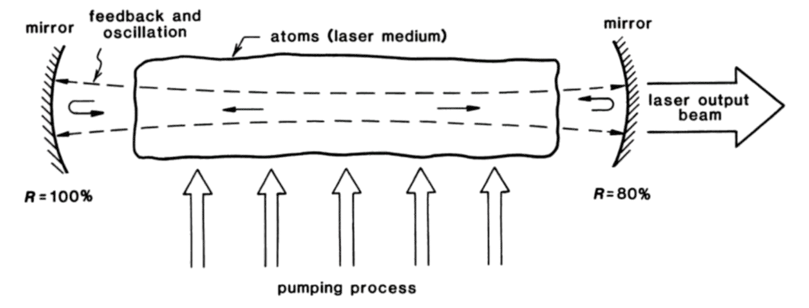
\includegraphics[width=0.8\textwidth]{images/width_809.png}
\end{center}

\begin{itemize}

    \item \textbf{Stimulated Emission:} When an atom or molecule in an excited state encounters a photon with energy equal to the transition energy to a lower state, it can be stimulated to emit a second photon identical in frequency, phase, polarization, and direction to the incident photon.

    \item \textbf{Population Inversion:} For stimulated emission to dominate over absorption, more atoms must occupy the excited state than the ground state a condition known as population inversion. This non-thermal equilibrium state is achieved through pumping, where external energy (electrical, optical, or other forms) excites the gain medium.

    \item \textbf{Optical Feedback:} An optical resonator (typically formed by two mirrors) provides positive feedback, allowing photons to make multiple passes through the gain medium, stimulating further emission. One mirror is partially transmissive, allowing a fraction of the amplified light to escape as the laser beam.
    

\end{itemize}

Some essential characteristics of lasers are: coherence, monochromaticity, directivity, and brightness.

\subsection{Why Do We Need Them For?}
In our case we will use Laser diodes due to their compactness, efficiency, direct electrical pumping, compatibility with specific atomic transitions such as Rubidium D-lines at 780 nm and 795 nm, tunability, and cost-effectiveness for laboratory use.
\\
The external cavity configuration we employ enhances the basic laser diode's performance by narrowing its linewidth and in near future enabling mode-hop-free tuning, making it suitable for precision spectroscopy and laser cooling experiments.

\section{Atomic Physics Experiments}
Lasers have changed experimental atomic physics by allowing precise spectroscopy and control of atomic systems. They are essential for exploring quantum phenomena, testing nature's symmetries, and advancing quantum technologies. This section discusses lasers' roles in measuring and manipulating atomic systems, focusing on alkali atoms and cold atoms.

\subsection{Alkali Atoms: Rubidium 85 and 87}
Rubidium is a soft, ductile alkali metal, composed naturally of two stable isotopes, 85Rb and 87Rb, in the following ratio; $72.15$ \% corresponds to 85Rb and $27.85$ \% to 87Rb. The D2 line of Rubidium 85 and 87 has a natural linewidth (FWHM) of $6.07$ MHz~\cite{steck85,steck87}, which is the transition we will use for cooling and trapping atoms in a Magneto\- Optical Trap (MOT). 

\begin{figure}[H]
    \begin{subfigure}{0.45\textwidth}
        \centering
        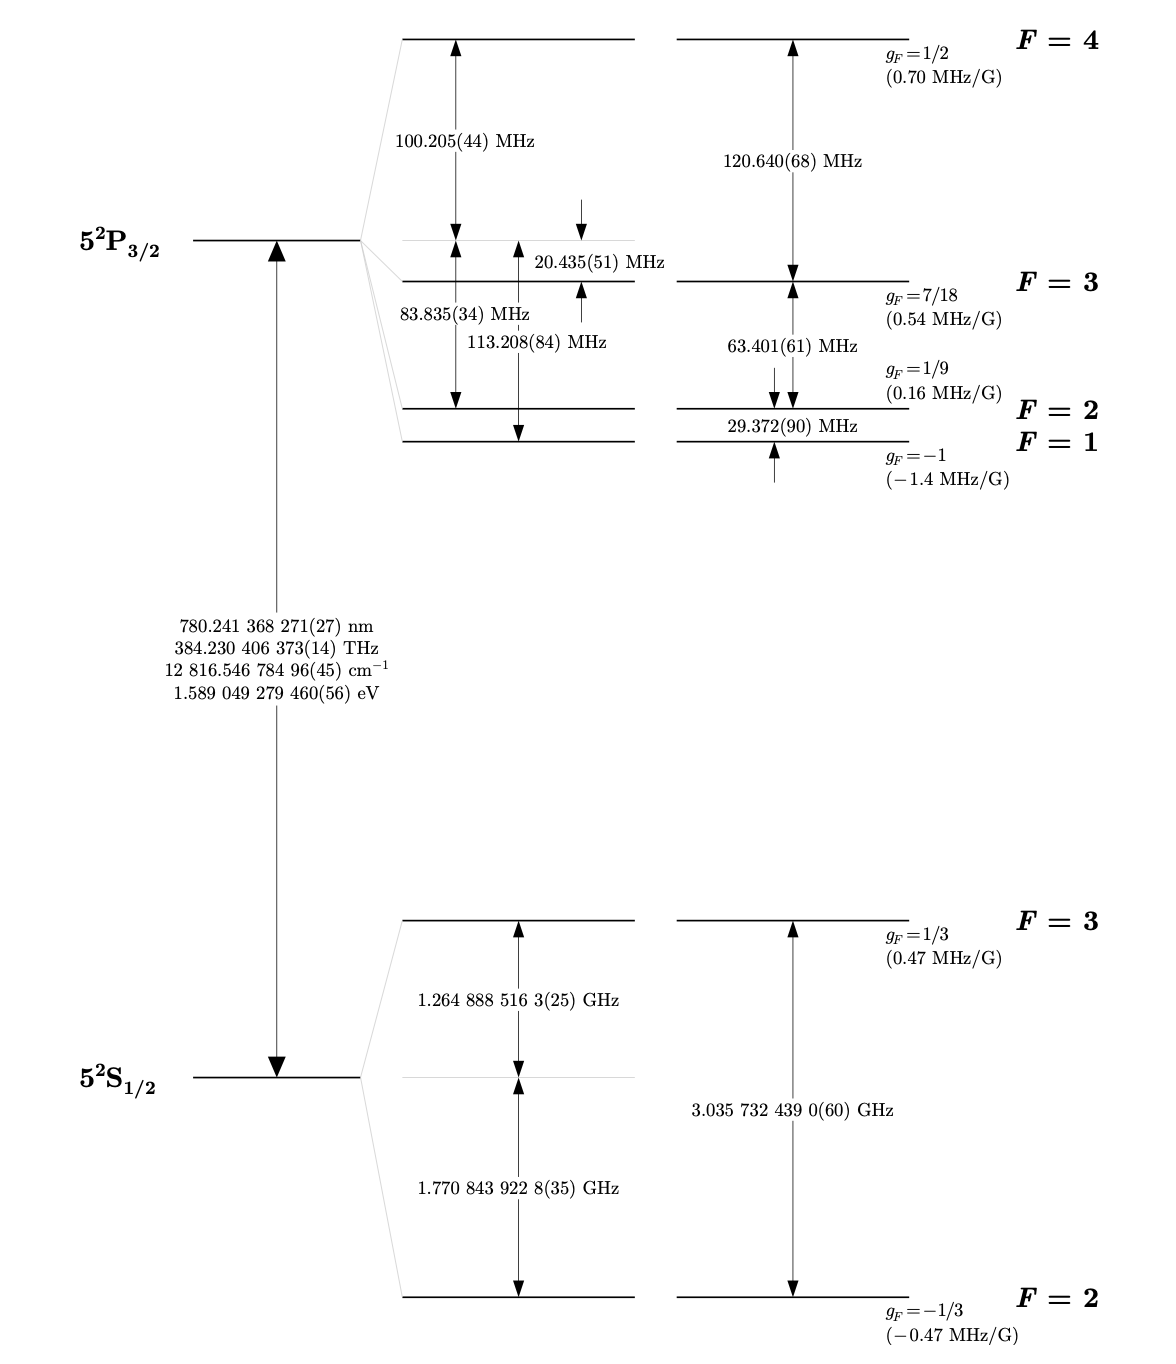
\includegraphics[width=0.8\textwidth]{images/rb85.png}
    \end{subfigure}
    \hfill
    \begin{subfigure}{0.45\textwidth}
        \centering
        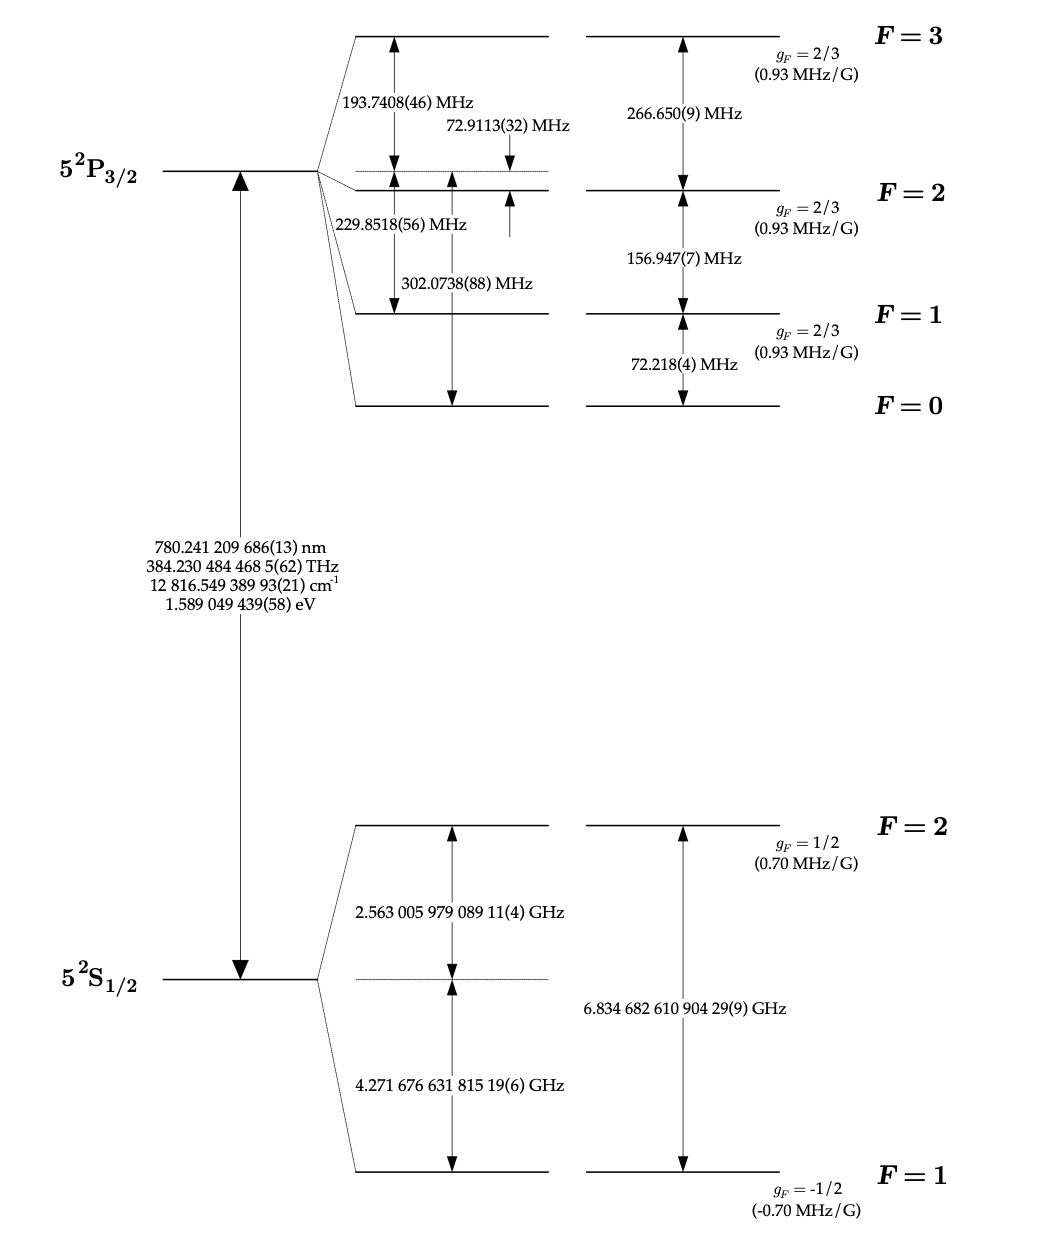
\includegraphics[width=0.8\textwidth]{images/rb87.png}
    \end{subfigure}
 \caption{Rubidium 85 and 87 D2 transition hyperfine structure, with frequency splittings between the hyperfine energy levels.}
\end{figure}

\subsection{Laser Cooling and Trapping of Atoms}

Laser cooling uses light-matter momentum transfer to slow atomic motion, achieving temperatures as low as microkelvin. In Doppler cooling, the foundational technique, counter-propagating laser beams tuned slightly below an atomic resonance (e.g., Rb-87’s D$_2$~line at 780~nm) create a velocity-dependent damping force that reduces kinetic energy~\cite{foot}. This cooling enables optical molasses, where atoms scatter photons cyclically, reaching temperatures near the Doppler limit $T_D=\frac{\hbar \Gamma}{2 k_B}$~\cite{molasses}.
\medskip

\subsection{Magneto-Optical Trap (MOT)}
For trapping, magneto-optical traps (MOTs) combine laser cooling with quadrupole magnetic fields to confine atoms at densities up to $10^8 $atoms/cm$^3$~\cite{Phillips}. The MOT uses six laser beams arranged symmetrically around the trap center, tuned to the red of the atomic resonance, and a magnetic field gradient to create a restoring force that arises from Zeeman shift enhanced scattering in regions of non-zero field gradient, creating a net restoring force toward the trap center. Radiation pressure from the lasers balances this force, enabling stable, long-term confinement of ultracold atomic ensembles~\cite{Rabb}.

\begin{figure}[ht]
    \centering
    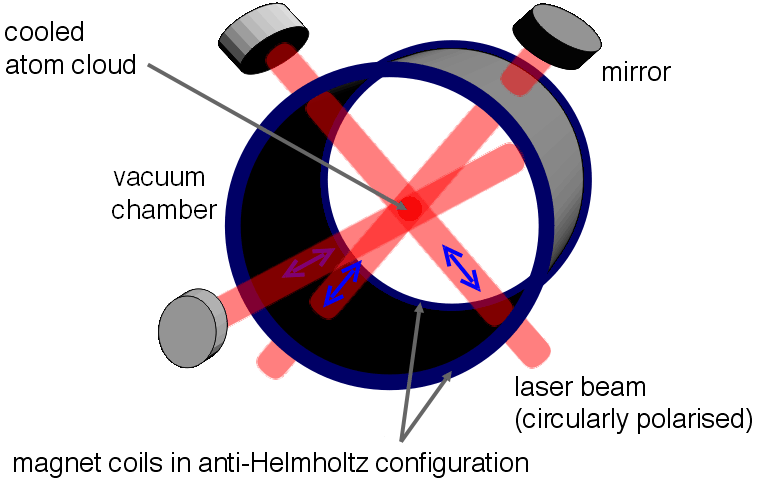
\includegraphics[width=0.6\textwidth]{images/MOT_setup.png}
    \caption{Magneto-Optical Trap (MOT) setup~\cite{MOTsetup}.}\label{fig:MOT_setup}
\end{figure}
Critical to both Doppler cooling and MOT confinement is precise laser linewidth stability ($\Delta \nu < \Gamma \approx 6$ MHz for Rb-87) and intensity control. Narrow linewidth ensures resonant photon scattering for efficient momentum transfer, while stabilized intensity maximizes scattering rates without causing excessive heating or loss of atoms. Achieving these requirements necessitates advanced laser systems, often involving external cavity configurations and optical feedback techniques.
\section{How do we measure the linewidht of the laser: Self-Heterodyne Spectroscopy}
To measure the linewidth of our laser system, we employ self-heterodyne spectroscopy, a technique based on the Wiener-Khintchine theorem. This method involves splitting the laser beam into two paths—one delayed by a time $\tau$ relative to the other—and then recombining them on a photodetector. The interference pattern yields the power spectral density (PSD), which reveals the laser's coherence properties.

\begin{formal}
\textbf{Power Spectral Density Function:}
The PSD derived from the Wiener-Khintchine theorem for our setup is:
\begin{equation}
    S(\omega, \tau) = \frac{\frac{1}{2} P_0^2 \tau_c}{1 + {\omega \pm \Omega}^2 \tau_c^2} \left\{ 1 - e^{-\frac{-|\tau|}{\tau_c}} [\cos(\omega \pm \Omega)] \tau \right\} + \frac{\sin(\omega \pm \Omega) |\tau|}{(\omega \pm \Omega) \tau_c} + \frac{1}{2} P_0^2 \pi e^{-\frac{-|\tau|}{\tau_c}} \delta(\omega \pm \Omega)
\end{equation}
where $\tau_c$ is the coherence time, $\Omega$ is the frequency shift from an acousto-optic modulator (AOM), and $P_0$ is the laser power. This model predicts two regimes: when $\tau \gg \tau_c$, the spectrum collapses to a pure Lorentzian; when $\tau \ll \tau_c$, it shows a narrow delta function peak. Achieving sub-MHz linewidths typically requires fiber delays of tens of kilometers, which is impractical for most laboratories. Our approach uses optical feedback to achieve narrow linewidths without such long delays~\cite{Richter1986}.
\end{formal}

\begin{figure}[H]
    \centering
    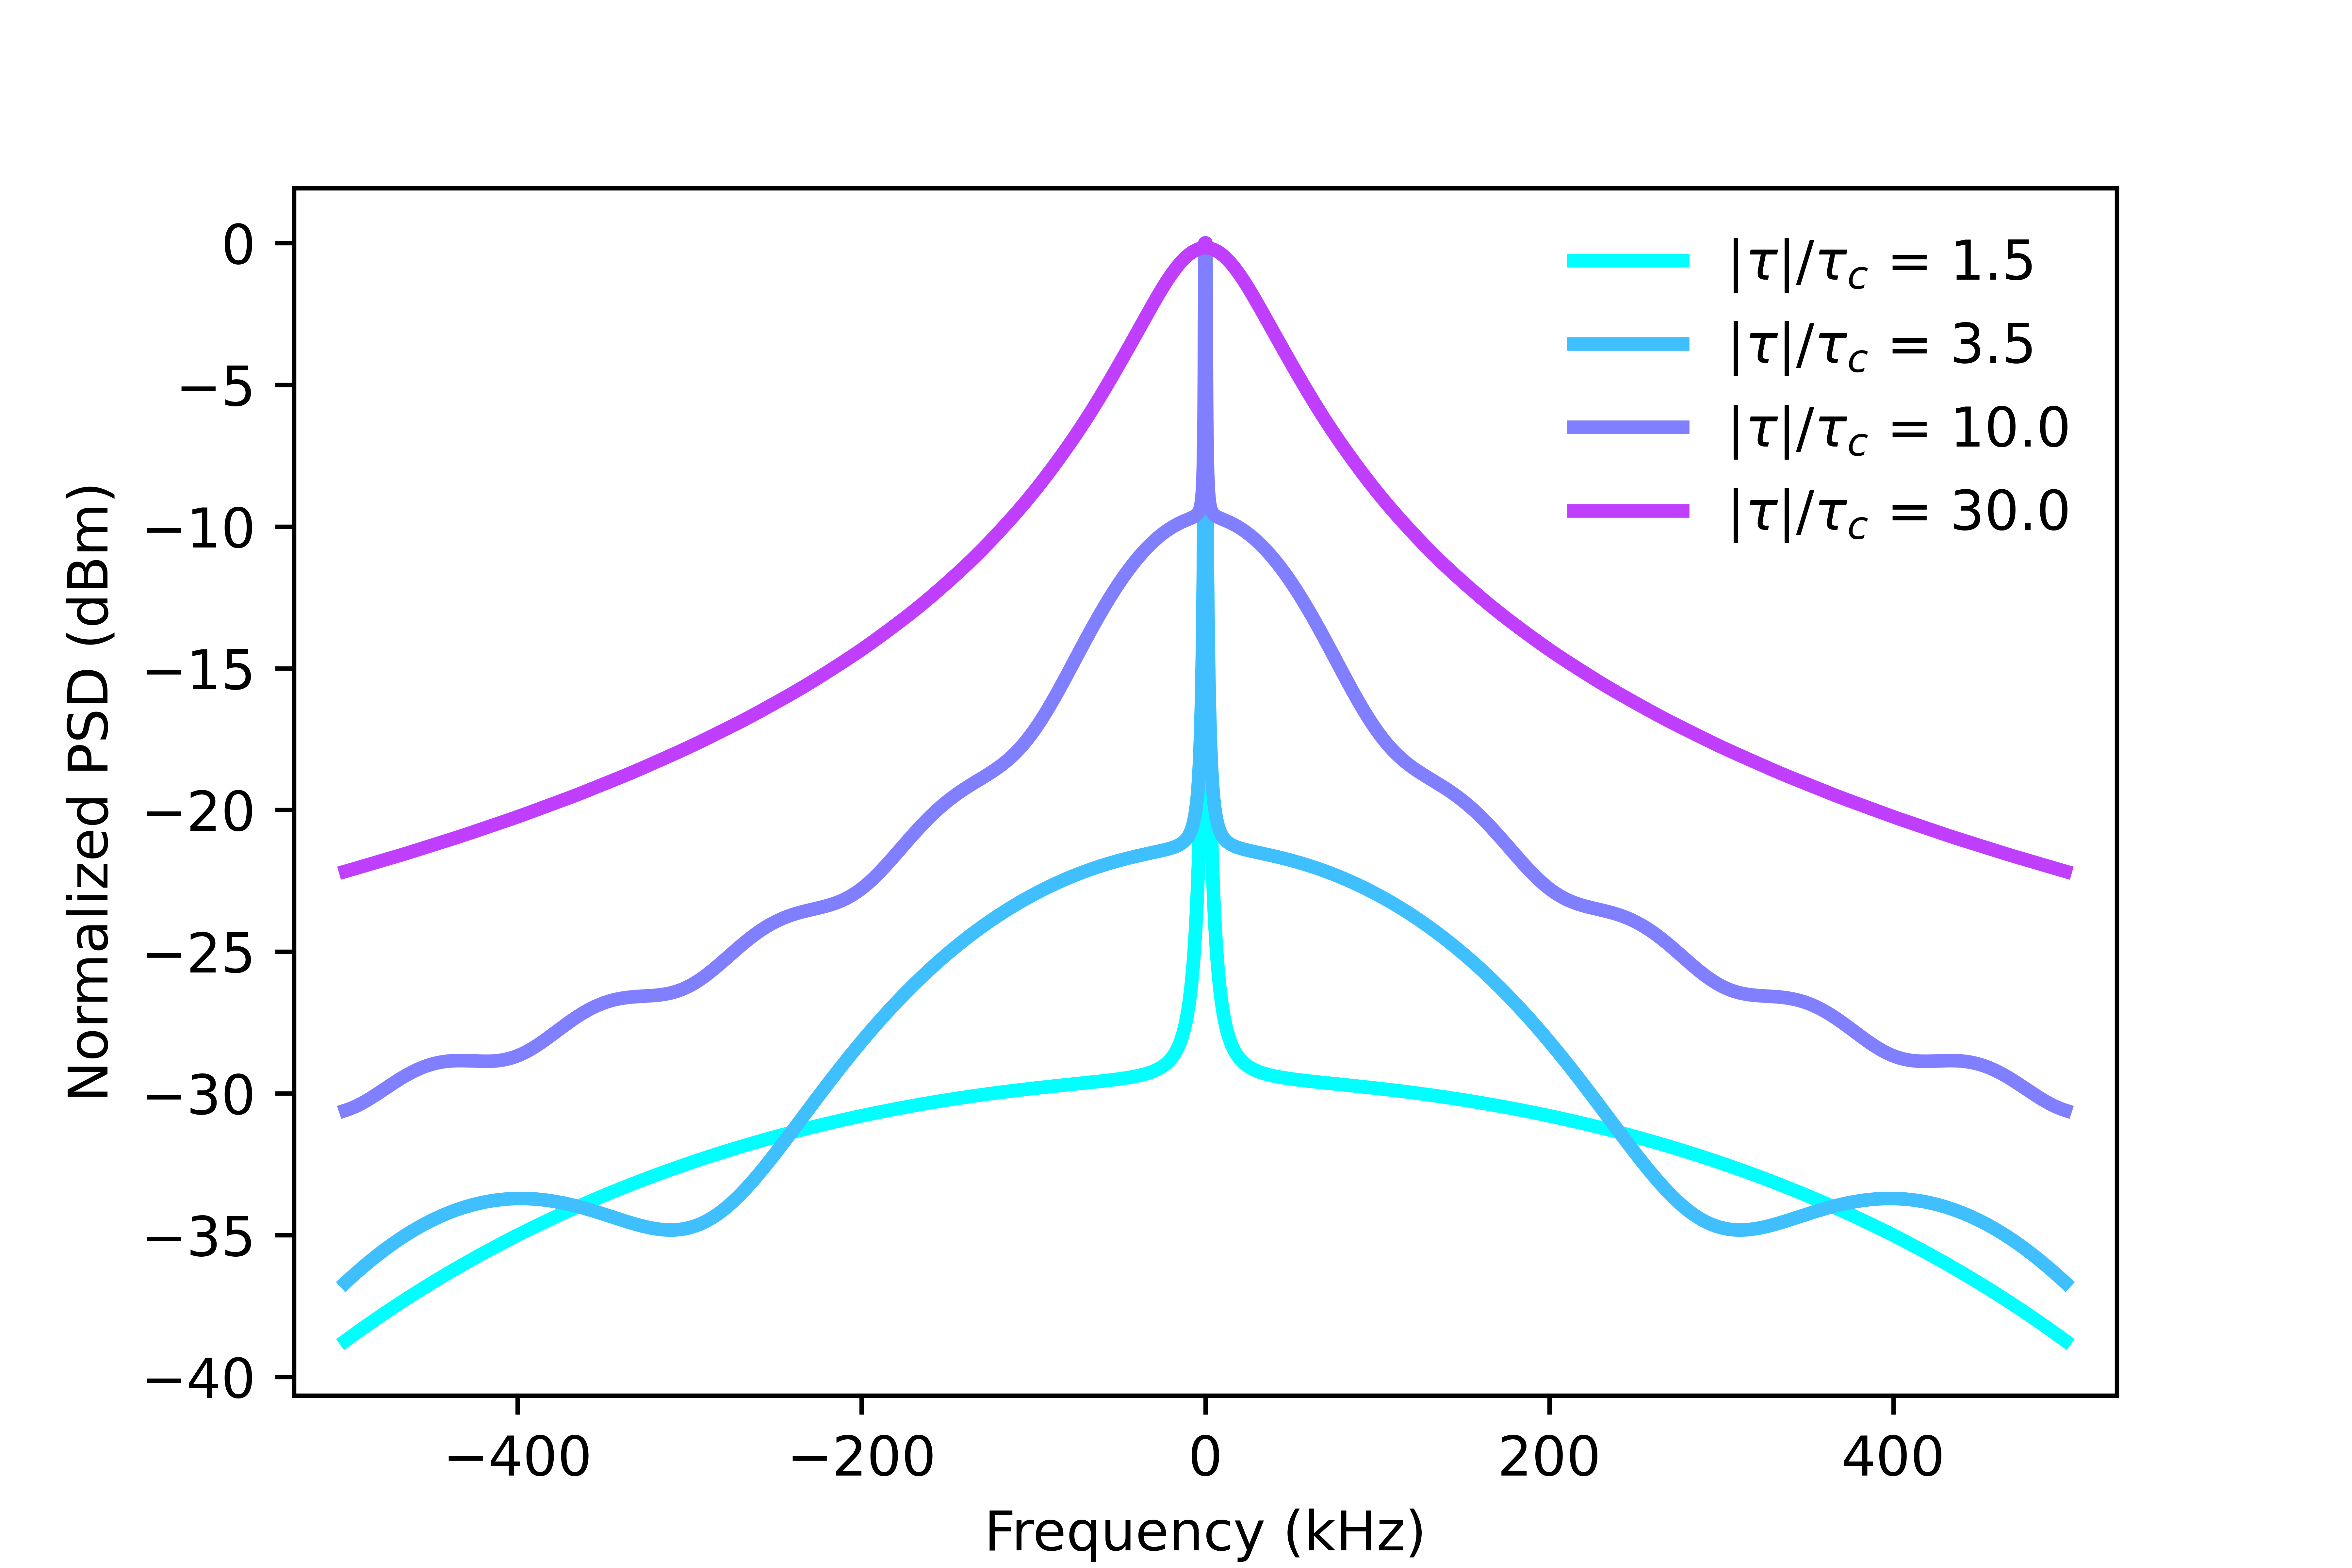
\includegraphics[width=0.8\textwidth]{images/PSD_simulation.png}
    \caption{Simulation of the power spectral density model in different regimes of coherence. The transition from coherent to incoherent interference is evident as the delay time increases relative to the coherence time.}\label{fig:psd_simulation}
\end{figure}

\section{How Can We Build Our Own Laser?}
The steps involved in creating a functional laser system are described in this section. It covers choosing components, circuit design, optical alignment, and optimization methods. The method seeks to address particular requirements for atomic physics experiments and emphasizes the integration of theory and practice.

\subsection{Electronics}
Electronic control systems are vital for stable laser systems, focusing on current regulation, temperature stabilization, and frequency locking. Key circuits include the current driver, temperature stabilization, and lock-in amplifier for reliable atomic physics experiments.\cite{scherz2016practical}

 \subsubsection{Basic Components: Resistance, Capacitance, Inductance}
Electronic circuits for laser control utilize three fundamental passive components:
\begin{itemize}
    \item \textbf{Resistors:} The characteristic by which it oppose the flow of current is known as resistance. The resistance of a resistor is denoted by symbol R and measured in Ohms ($\Omega$). The typical circuit symbol of a resistor is shown in the following figure.
    \begin{figure}[ht]
        \centering
        
\includegraphics[width=0.6\textwidth]{images/width_700.png}
    \end{figure}\\
    Resistors are used to set operating current and signal levels in circuits, provide voltage reduction, set precise gain values in precision circuits, act as shunts in ammeters and voltage meters, behave like damping agents in oscillators and timer circuits, act as bus and line terminators in digital circuits, provide feedback networks for amplifiers, and act as pull up and pull down elements in digital circuits.
        \begin{formal}
        \textbf{OHM's Law:}
        \\  The linear relationship between voltage ($V$), current ($I$), and resistance ($R$):
            \begin{equation}
                V = IR \nonumber
            \end{equation}
         This equation rule the current flow through resistive elements, allowing us to calculate voltage drops, power dissipation ($P = I^2R = V^2/R$). 
         
         %For AC circuits with reactive components (capacitors and inductors), this relationship extends to complex impedance ($Z$), where $V = IZ$, with impedance depending on frequency due to the phase shifts introduced by capacitance and inductance.

        \end{formal}

    \item \textbf{Capacitors:} Their major function is simple energy storage, where charge from an applied current is stored within the capacitor and later released back into the circuit as useful current. The rate of charging and discharging can be controlled by placing a resistor in series with the capacitor. This effect is often used in high-current discharge circuits, as well as small energy backup supplies for low-power memory Integrated circuits(ICs). It is also used to smooth out power supply ripple, control timing in ICs, and alter the shape of waveforms.
    
    \begin{figure}[h!]
        \centering
        
\includegraphics[width=0.6\textwidth]{images/cap.png}
    \end{figure}

    
    \item \textbf{Inductors:} The inductor is basically a wire of finite length twisted into a coil and has a property, known as inductance, which oppose any change in the electric current.
   
    \begin{figure}[h!]
        \centering
        
\includegraphics[width=0.6\textwidth]{images/indu.png}
    \end{figure}

    \begin{formal}
        \textbf{Inductance:}
        The voltage across an inductor is proportional to the rate at which the current changes. The relationship between voltage and current are described by the following equations:
        \begin{equation}
            V_L = L \frac{dI_L}{dt} 
        \end{equation}
        
        \begin{equation}
            I_L= \frac{1}{L}\int V_L
        \end{equation}

    \end{formal}
\end{itemize}

\subsubsection{Active components}
 Active components control current flow and amplify signals using external power sources, enabling precise laser regulation.

\begin{itemize}
    \item \textbf{Semiconductors:}
    A semiconductor is a material whose electrical conductivity lies between a conductor and an insulator. This unique property makes semiconductors ideal for controlling electrical current, enabling their use in a wide range of electronic devices. 
    \begin{itemize}
        \item \textbf{Diodes:} A two-lead semiconductor device that acts as a one-way gate to electric current flow. When a diode’s anode lead is made more positive in voltage than its cathode lead the condition is referred to as forward biasing so the current is permitted to flow through the device.
        
        \begin{figure}[h!]
            \centering
            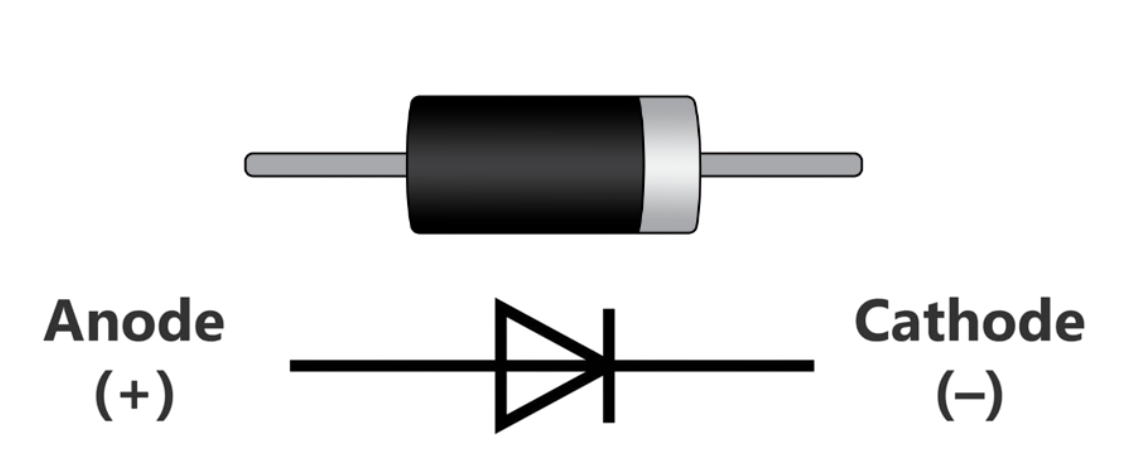
\includegraphics[width=0.4\textwidth]{images/diode.png}
        \end{figure}
        
        \item \textbf{Transistors:} Three-terminal semiconductor devices that amplify or switch electronic signals. Bipolar Junction Transistors (BJTs) are current-controlled and excel in linear, low-noise applications like current regulators, while Metal-Oxide-Semiconductor Field-Effect Transistors (MOSFETs) are voltage-controlled and offer fast switching with minimal gate current, ideal for pulse-width modulation (PWM) in temperature controllers.
        
        \begin{figure}[ht!]
                \centering
                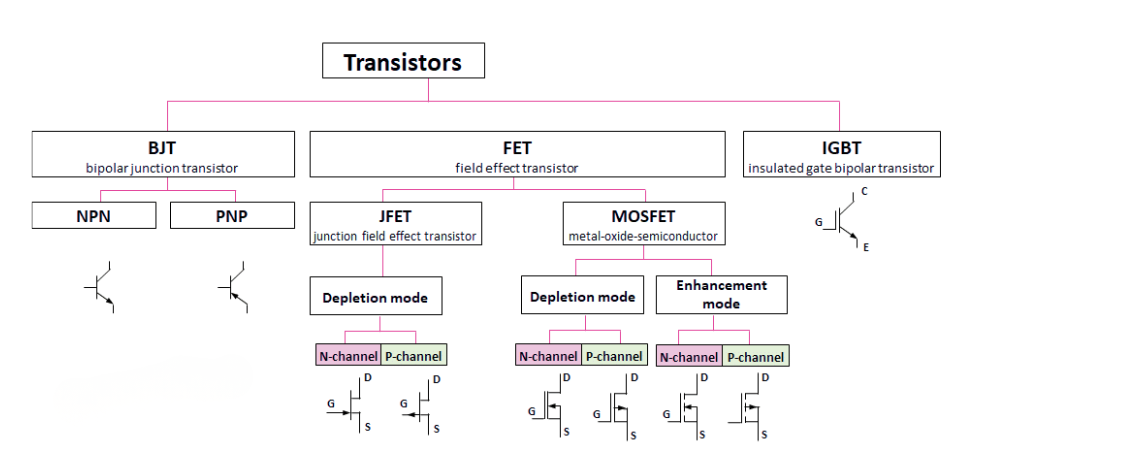
\includegraphics[width=0.75\textwidth,right]{images/Transistores.png}
        \end{figure}
            
    \end{itemize}
    \item \textbf{Amplifiers:} They are essential circuits for increasing signal amplitude while preserving signal integrity, playing critical roles in laser control systems for error signal processing, photodetector signal conditioning, and driving control elements.
    
    \begin{itemize}
        \item \textbf{Operational Amplifiers:} Op amps are high gain differential amplifiers with two inputs (inverting and non-inverting) and a single output. In ideal behavior, they have infinite open loop gain, infinite input impedance, zero output impedance, and infinite bandwidth. Real op amps approach these ideals with specifications tailored to specific applications.
        
        \begin{figure}[H]
                \centering
                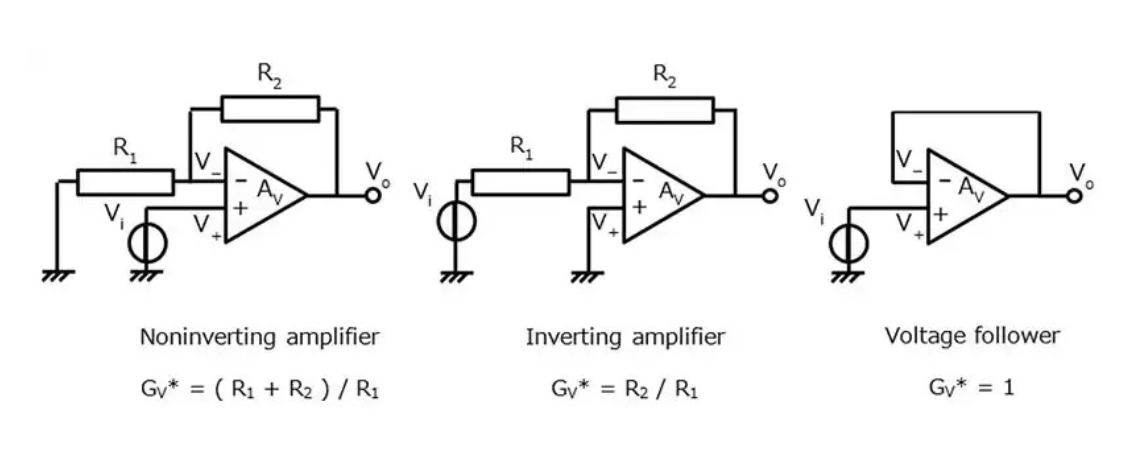
\includegraphics[width=0.75\textwidth,right]{images/Oamp.png}
        \end{figure}

        \begin{formal}
            \textbf{Gain:} The amplification factor of a circuit, defined as the ratio of output to input signal. For voltage amplifiers, $A_v = V_{out}/V_{in}$; in decibels, $G_{dB} = 20\log_{10}(A_v)$. Determines sensitivity of feedback loops and must be optimized for stability versus response speed.
        \end{formal}

        \item \textbf{Instrumental Amplifiers:} INAmp is a high precision differential amplifier designed to amplify small signals from sensors while rejecting common mode noise, featuring high input impedance, high gain, and excellent common mode rejection ratio (CMRR).
        
    \end{itemize}

    
\end{itemize}
 



\subsubsection{Low and high pass filters:}
Low-pass and high-pass filters are essential for controlling a signal's frequency content. A low-pass filter allows low-frequency signals to pass through while reducing the amplitude of higher-frequency signals, and a high-pass filter does the opposite, allowing high frequencies to pass through while blocking low-frequency components. 


\begin{figure}[ht!]
        \centering
        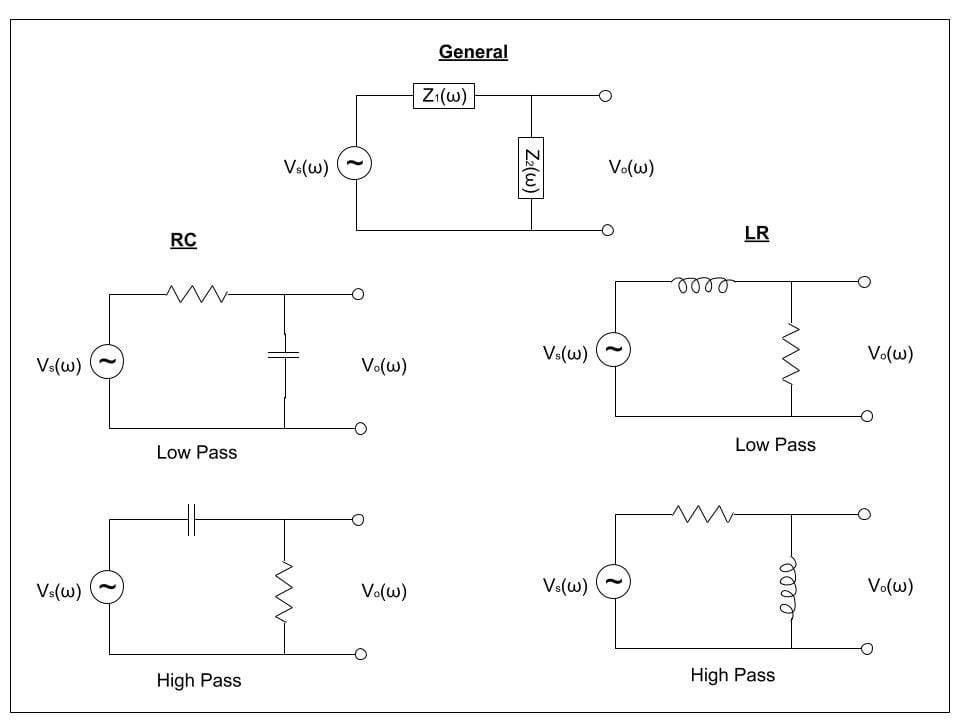
\includegraphics[width=0.6\textwidth]{images/low-and-high-pass-1cg8gnq.jpg}
        \caption{ The low and high-pass versions of the RL and RC circuits. $V_s(w)$ is the voltage of the function generator and $V_o(w)$ is the voltage on the oscilloscope.}
    \end{figure}


\begin{formal}
    \textbf{Impedance ($Z$):} generalizes resistance to AC circuits, representing the total opposition a circuit presents to alternating current flow. While resistance dissipates energy as heat, impedance includes both resistive and reactive components which store and release energy without dissipation. In complex notation, $Z = R + jX$, where $X$ is the reactance that depends on frequency: capacitive reactance $X_C = -1/(\omega C)$ decreases with frequency, while inductive reactance $X_L = \omega L$ increases.
\end{formal}

\subsection{Optoelectronics: Laser Diodes}

Laser diodes are light emitting diodes with two “mirrors” on the surface of the diode to create a laser cavity. When the diode is forward biased, charges are injected into the active area of the junction, while electrons and holes recombine in the junction, creating spontaneous emission of photons. These photons can cause other electron hole pairs to recombine by stimulated emission. When the current is high enough, the device lases.\cite{Paschotta_2005_laser_diodes} 

\begin{figure}[ht!]
        \centering
        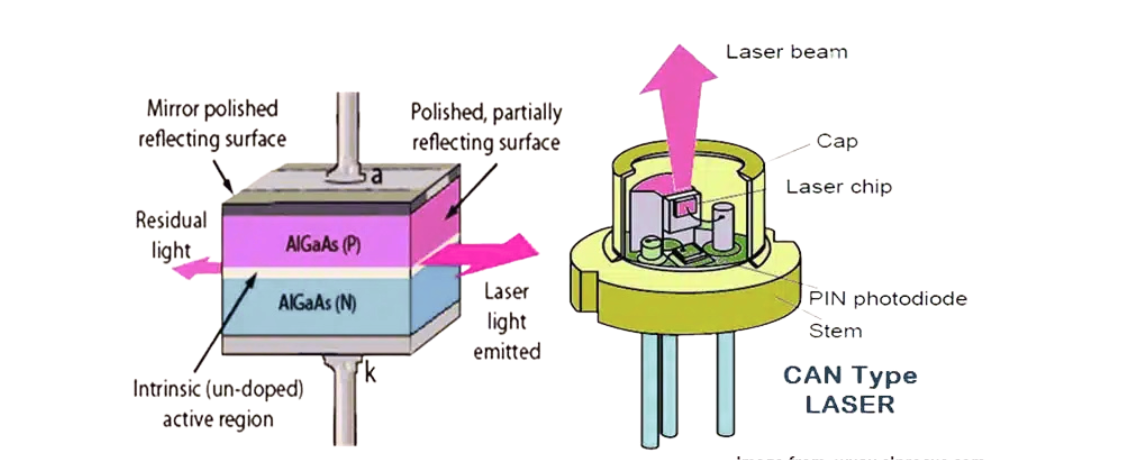
\includegraphics[width=0.6\textwidth]{images/laserdiode.png}
    \end{figure}

\subsection{Hands-On Construction}

The electronic control system is constructed from four independent but interconnected circuits, each addressing a specific aspect of laser stabilization. All circuits are built on custom designed printed circuit boards (PCBs) to minimize noise, improve reliability, and facilitate troubleshooting.

\subsubsection{Negative Current Control Circuit:}
The laser diode driver requires precise, low noise current regulation. We implement a negative feedback current controller\footnote{For more details of the ncc circuit see APPENDIX ~\ref{apx}} that maintains constant current despite fluctuations in diode voltage and temperature.

\begin{figure}[h!]
        \centering
        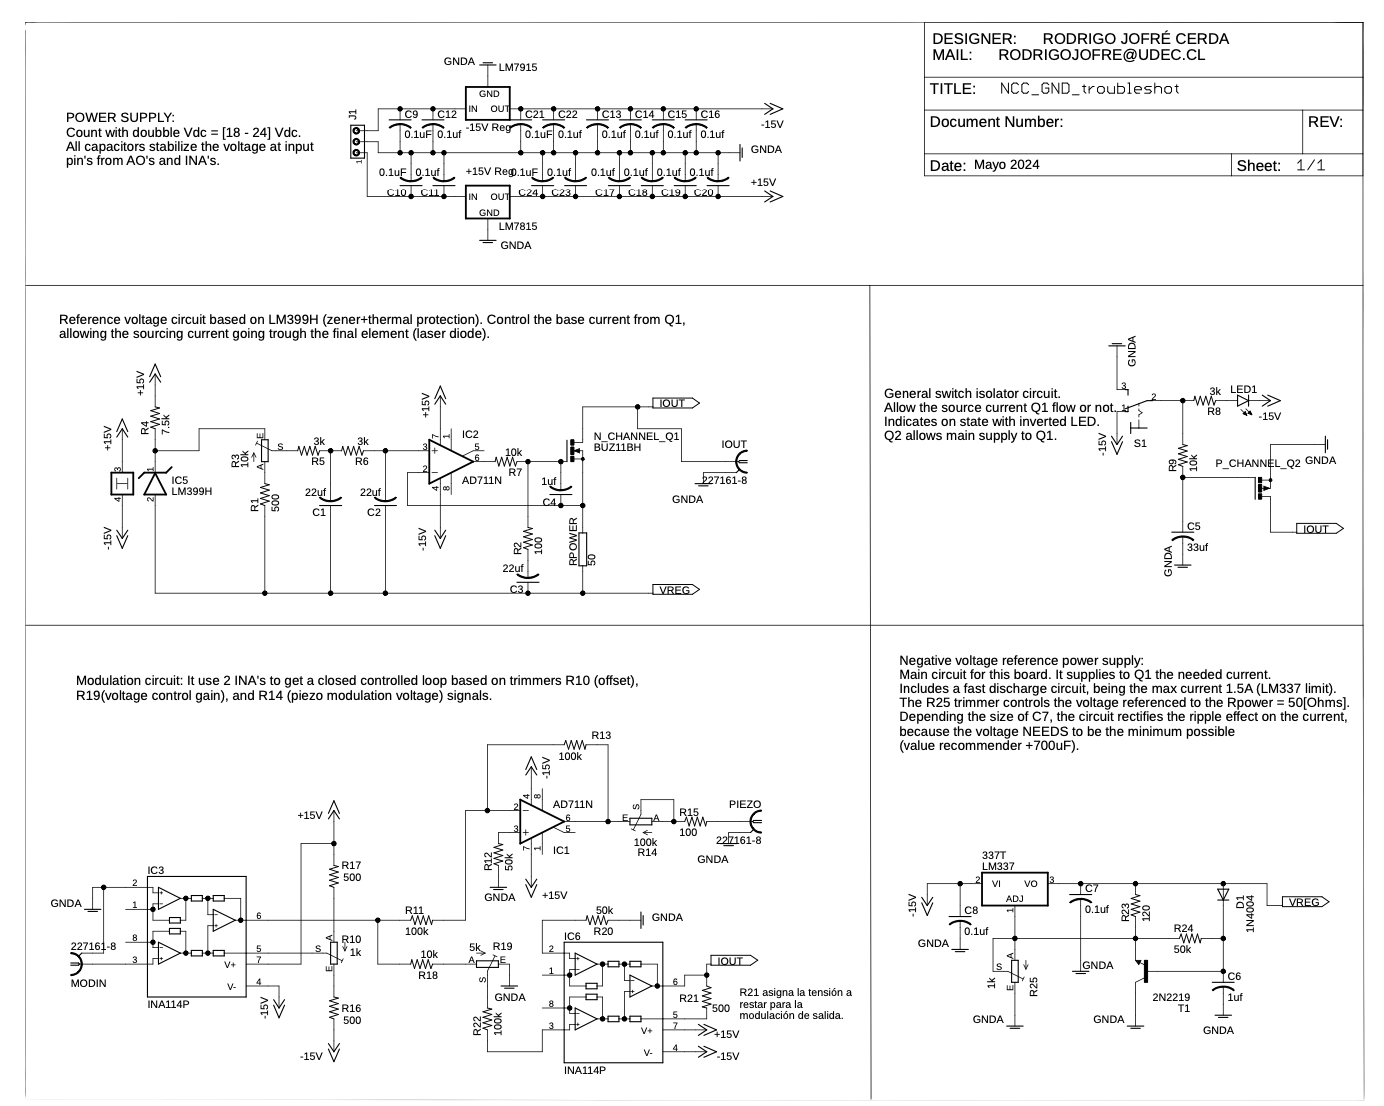
\includegraphics[width=0.7\textwidth]{images/width_1384.png}
\end{figure}

\subsubsection{Thermoelectric Circuit:}
Temperature stabilization is critical for wavelength control, as diode wavelength shifts approximately 0.3 nm/\(^\circ C\). We designed a thermoelectric cooler (TEC) controller using a dual operational amplifier
configuration. The first stage amplifies the voltage difference between a thermistor and a reference voltage, producing an error signal. The second stage, with adjustable gain, drives the TEC to maintain the laser diode at a constant temperature. The circuit includes protection diodes to prevent reverse current and large capacitors to stabilize the control voltage.

\begin{figure}[H]
    \centering
    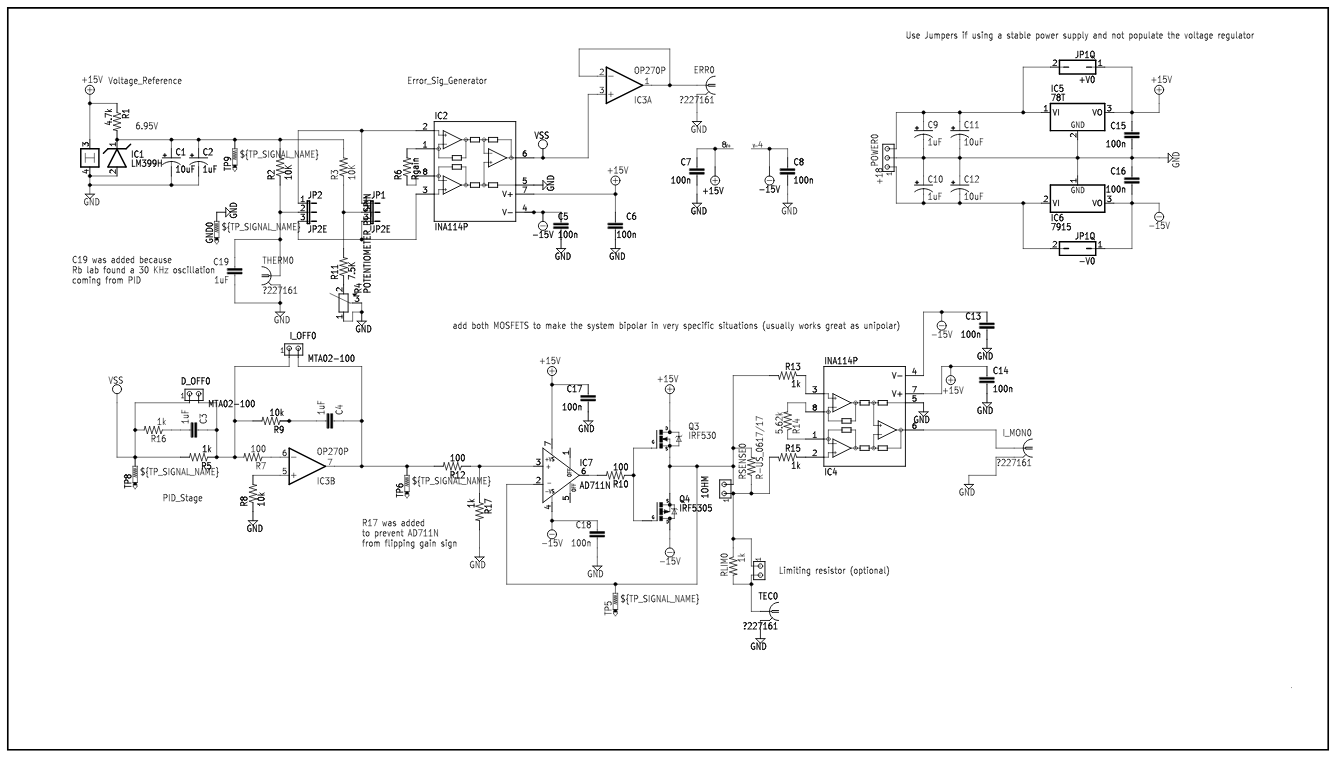
\includegraphics[width=0.9\textwidth]{images/TEC_circuit.png}
    \caption{Thermoelectric control circuit.}\label{fig:tec_circuit}
\end{figure}

\subsubsection{PID controller circuit:}
The PID circuit is often utilized as a control loop feedback controller. The letters making up the acronym PID correspond to Proportional (P), Integral (I), and Derivative (D), which represents the three control settings of a PID circuit. The PID circuit actively controls the system so as to hold it at the set point by generating an error signal that is essentially the difference between the set point and the current value. The three controls relate to the time-dependent error signal.
%https://www.thorlabs.com/driver-pid-settings?tabName=PID%2520Tutorial

\begin{figure}[H]
    \centering
    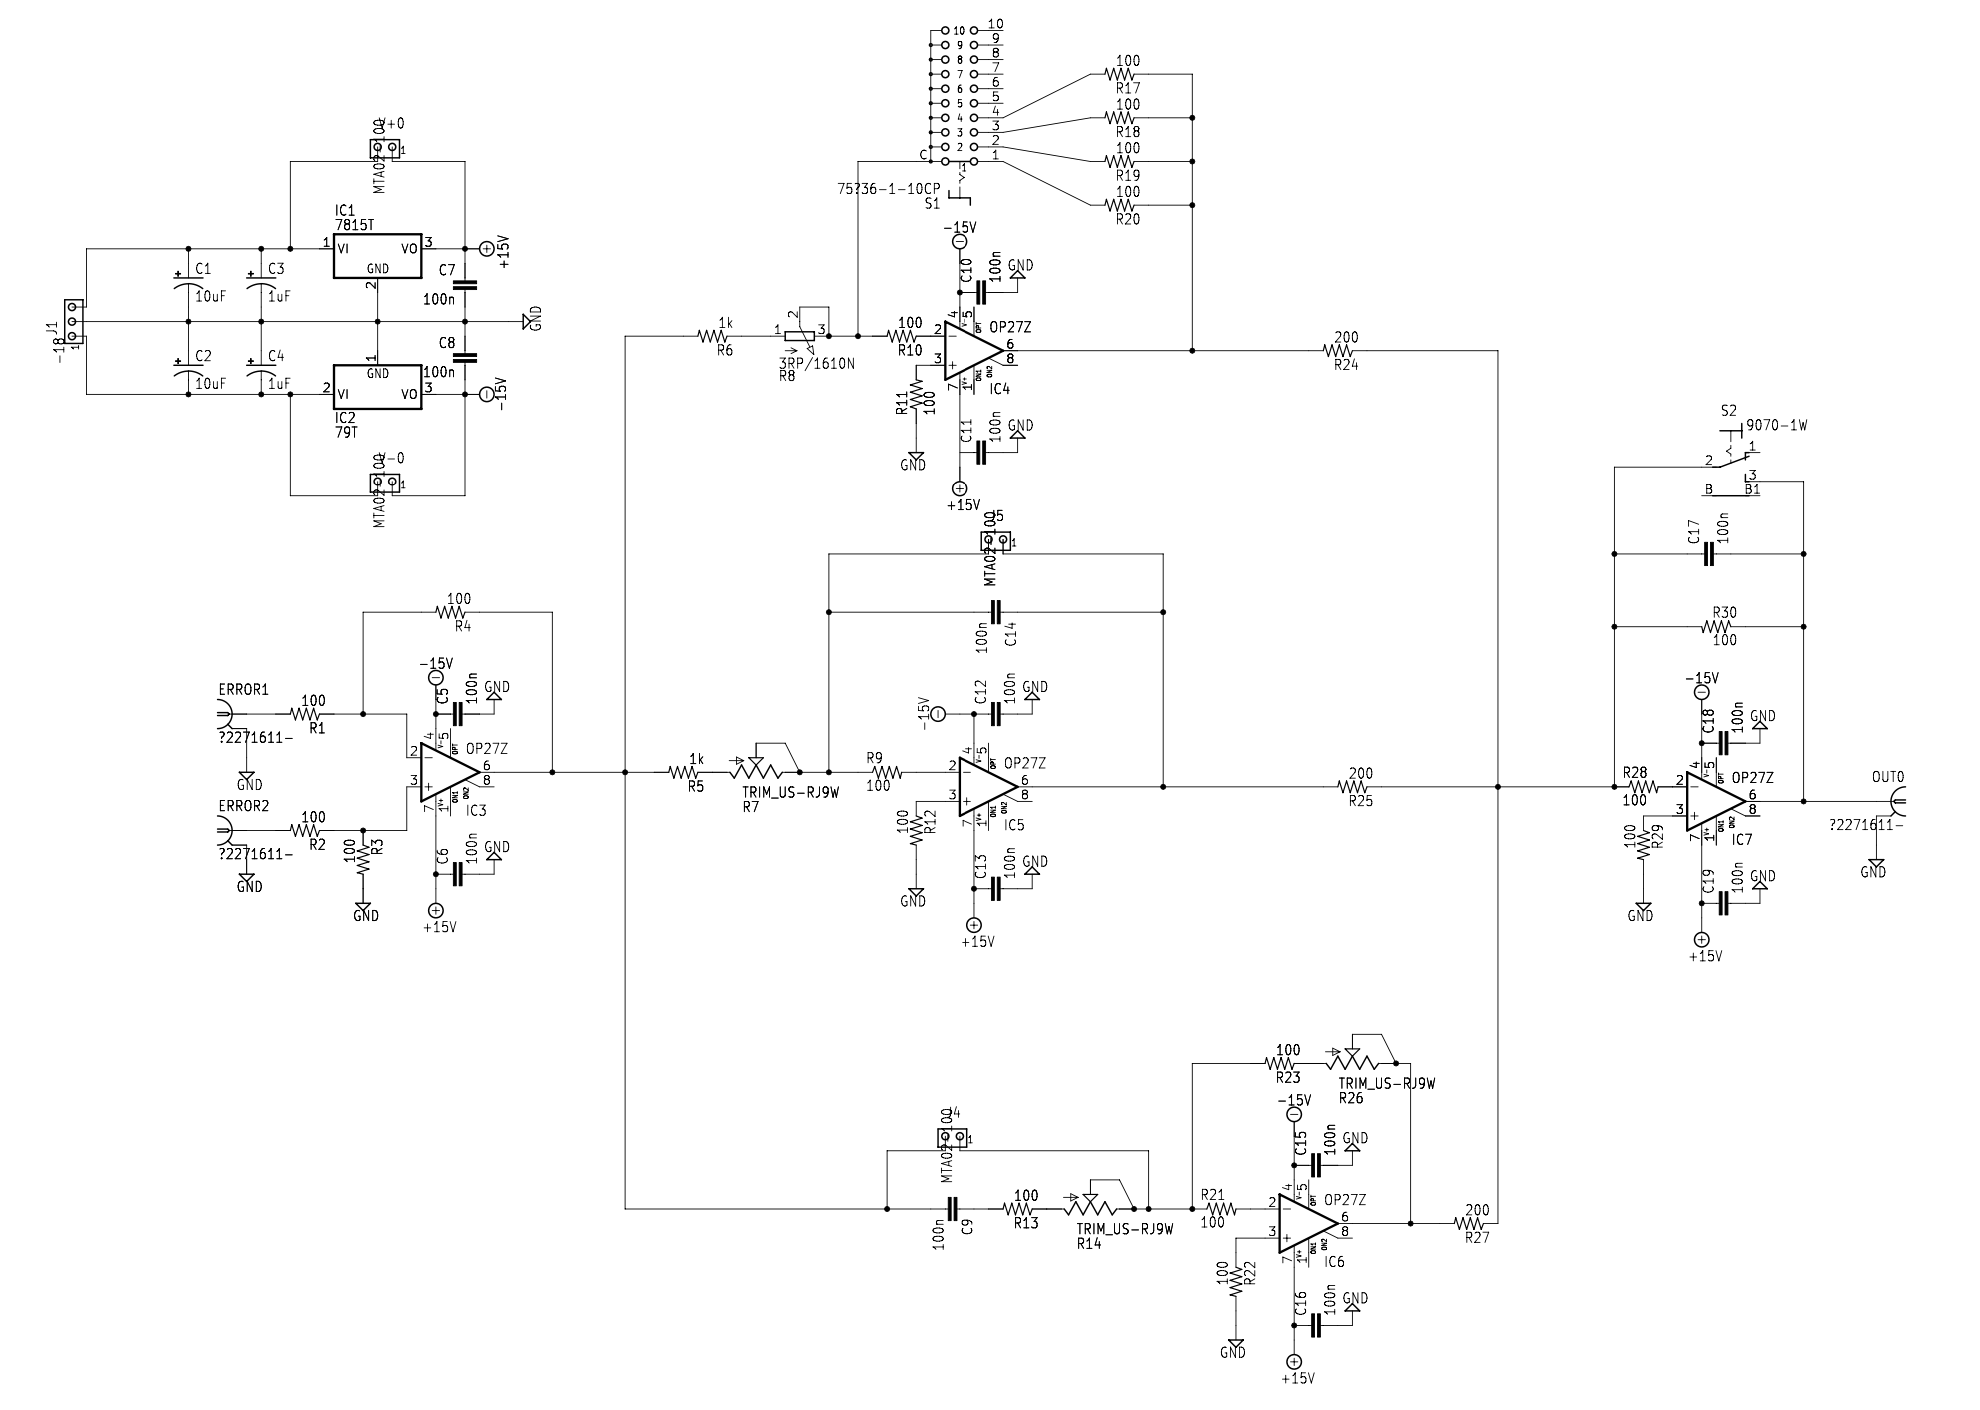
\includegraphics[width=0.9\textwidth]{images/PID_controller.png}
    \caption{PID controller circuit.}\label{fig:pid_circuit}
\end{figure}

\subsubsection{Lock-in Circuit:}
This circuit extracts the error signal from reflected laser light by mixing it with a reference
modulation frequency.

\begin{figure}[H] 
    \centering 
    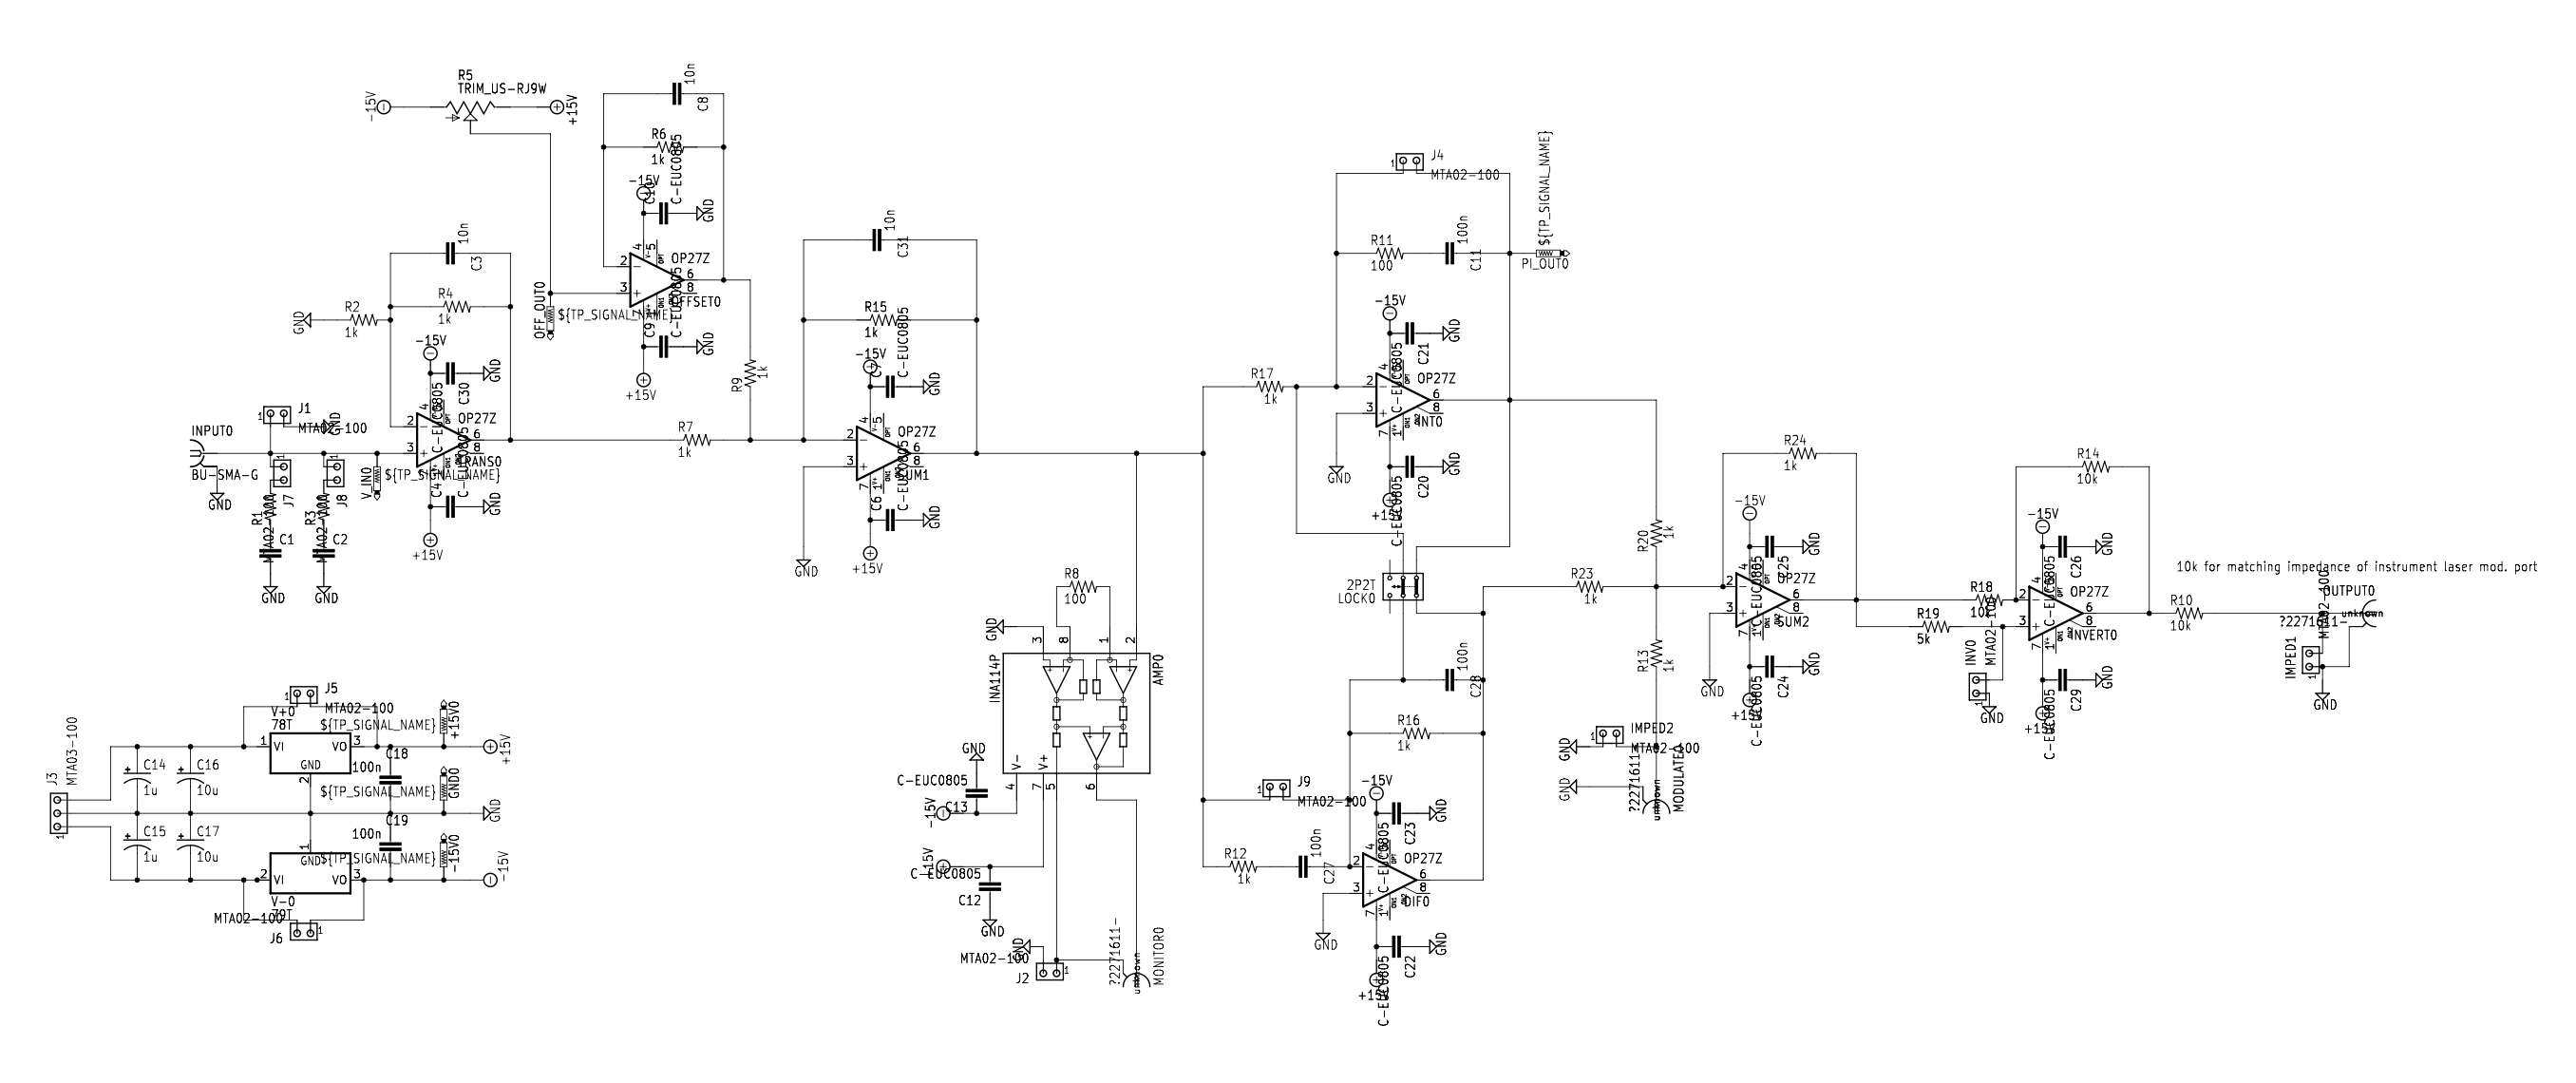
\includegraphics[width=0.7\textwidth]{images/lockbox_png.png}
    \caption{Lock-in amplifier circuit}\label{fig:lockin_circuit} 
\end{figure}

\subsubsection{PCB Design and Soldering:}
    All circuits were fabricated on custom-designed printed circuit boards (PCBs) to minimize noise and ensure reliability. Soldering was performed using a temperature-controlled soldering iron  with proper flux application. Sensitive components like the laser diode were soldered quickly to prevent thermal damage. 

\section{Optics:}
\subsection{Optical elements}
    Our laser system employs several key optical components:
    \begin{itemize}
        \item \textbf{Diffraction grating:} is an optical device exploiting the phenomenon of diffraction. It contains a periodic structure, which causes spatially varying optical amplitude and/or phase changes.\cite{Paschotta_2013_diffraction_gratings}
        \item \textbf{Beam splitter:} They separate incident light into two or more beams of the same wavelength. 
        \item \textbf{Acusto-Optic Modulator(AOM):} is a device which can be used for controlling the transmitted power of a laser beam with an electrical drive signal.\cite{Paschotta_2019_acousto_optic_modulators}
        \item \textbf{Piezoelectric transducer (PZT):} For fine adjustment of grating angle, the crystals produce a pressure when deformed by an applied voltage and produce a voltage when deformed by an applied pressure
        \item \textbf{Photodetectors:} Sensors that convert incident light into measurable electrical signals.
    \end{itemize}

\subsection{Narrowing the Linewidth}
% chktex 39

\subsubsection{External Cavity in a Laser Diode:} 
    We extended the laser cavity externally by adding a diffraction grating, which provides wavelength selective feedback. The external cavity length  increases the photon lifetime in the cavity, effectively narrowing the linewidth. 

\subsubsection{Optical Feedback:} 
    Controlled optical feedback from the diffraction grating narrows the linewidth through regenerative amplification. We optimized the feedback ratio to approximately $10-30$ \% of the output power. Too little feedback provides insufficient narrowing, while too much can cause instability or mode hops.

\subsection{Experimental Setup}
    \begin{figure}[H]
        \centering
        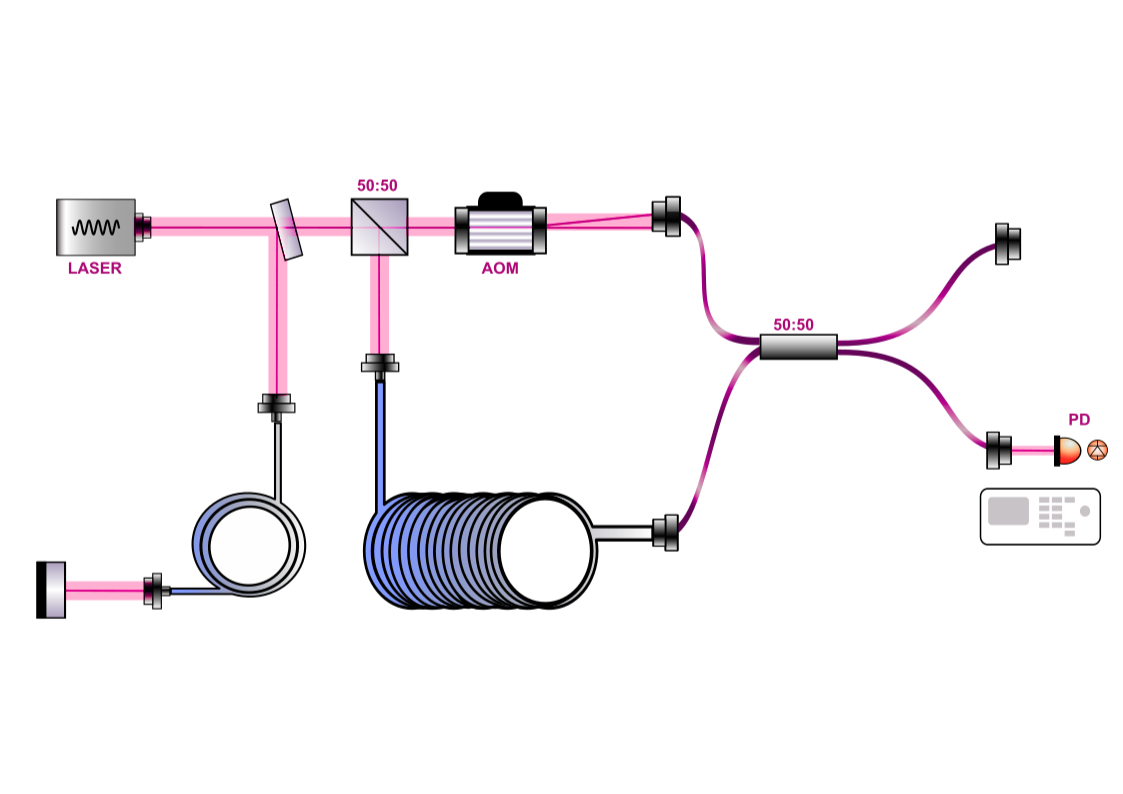
\includegraphics[width=0.7\textwidth]{images/exp_setup.png}
        \caption{Schematic representation of the experimental setup for feedback stabilized diode laser.}\label{fig:experimental_setup}
    \end{figure}


% \subsubsection{Littrow Configuration:} 
%     T1he Littrow is where the first\- order diffraction returns directly to the diode, maximizing efficiency. The grating equation for this configuration is:

%         \begin{equation}
%             \lambda = \frac{2d}{m} \sin\theta
%         \end{equation}

% where $d$ is the grating period (556 nm for 1800 lines/mm), $m$ is the diffraction order (1), and $\theta$ is the incidence angle ($\approx$ 45° for 780 nm).

%\subsubsection{Mode-Hop-Free Tuning:} 

% ===============================
% RESULTS SECTION
% ===============================
\section{Results}

We successfully constructed and characterized our in-house laser system, focusing on linewidth reduction through optical feedback stabilization. The performance was quantified using self-heterodyne spectroscopy with a fiber delay, allowing precise measurement of the laser's power spectral density (PSD) and coherence time.

\begin{figure}[H]
    \begin{subfigure}{0.45\textwidth}
        \centering
        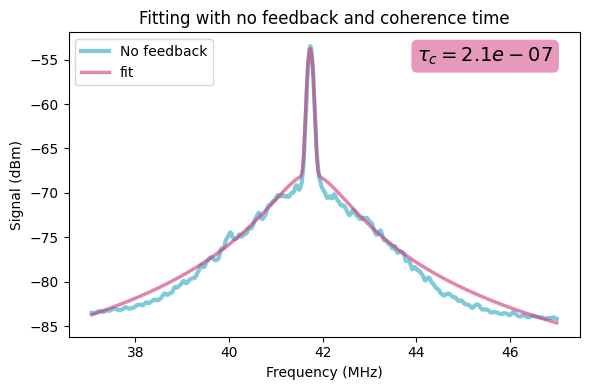
\includegraphics[width=0.8\textwidth]{images/nofeed.png}
        \caption{Without feedback}
    \end{subfigure}
    \hfill
    \begin{subfigure}{0.45\textwidth}
        \centering
        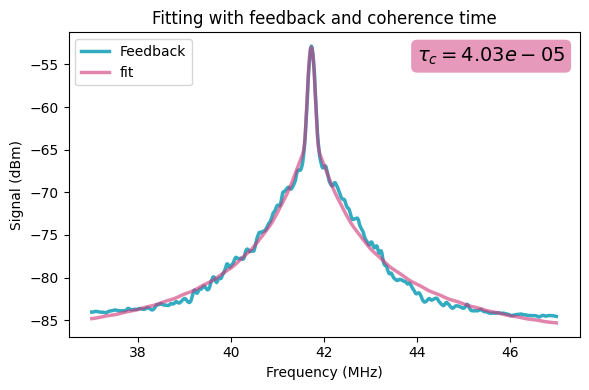
\includegraphics[width=0.8\textwidth]{images/feed.png}
        \caption{Width feedback}
    \end{subfigure}
 \caption{Measured power spectral density (PSD).}
\end{figure}

The coherence time $\tau_c$ increased from $2.1\times 10^{-7}$ s (without feedback) to $4.03\times 10^{-5}$ s (with feedback), corresponding to coherence lengths of 63 m and 12.1 km, respectively. This dramatic improvement enables precise spectroscopy of rubidium's hyperfine transitions.


% ===============================
% CONCLUSION SECTION
% ===============================
\section{Conclusion}

We have successfully designed, constructed, and characterized an in-house, low-cost, optically feedback stabilized diode laser system suitable for atomic physics experiments. Our work demonstrates that resource constrained laboratories can develop high performance laser systems through careful design and integration of commercial components. Future work will focus on integrating the laser into a complete magneto-optical trap system.

\vfill
\begin{flushright}
    \begin{tikzpicture}
        \duck[body=pink, unicorn=magenta!60!violet, longhair=magenta!60!violet, signpost=\parbox{2cm}{\tiny\color{black}\centering Bye! }, signcolour=brown!70!gray, signback=white!80!purple, shift={(2.5,0)}]      
\end{tikzpicture}
\end{flushright}

\newpage
% ===============================
% REFERENCES SECTION
% ===============================
\section*{References}
\addcontentsline{toc}{section}{References}
% Add your bibliography entries here
%\nocite{*}
\printbibliography[heading=none]
\newpage
% ===============================

%\noindent\makebox[\linewidth]{\rule{\paperwidth}{0.4pt}}
%\notebox{aaaaa}
%\awesomebox{5pt}{\faCertificate}{magenta}{aaa}
%\pgfornament[color=Mahogany,width=2cm]{8}
%
% APPENDIX (Optional)
% ===============================
\appendix~\label{apx}
\addcontentsline{toc}{section}{APPENDIX}
\paragraph{\Huge APPENDIX}
\section{Circuit Diagrams NCC:}
\subsection{Controlled dual power source (PS):}\label{ps}
 This setup uses two reference voltages to send the right amount of current to the Peltier system, which helps control the temperature.The circuit can provide strong output power. Each IC5 and IC6, which are integrated circuits, can handle up to 1.5A of current, or 3A total for the whole circuit, when the voltage is 18 volts direct current.Capacitors are included to keep the voltage signals steady for the main ICs in the industrial control system.

    \begin{figure}[ht!]
            \centering
            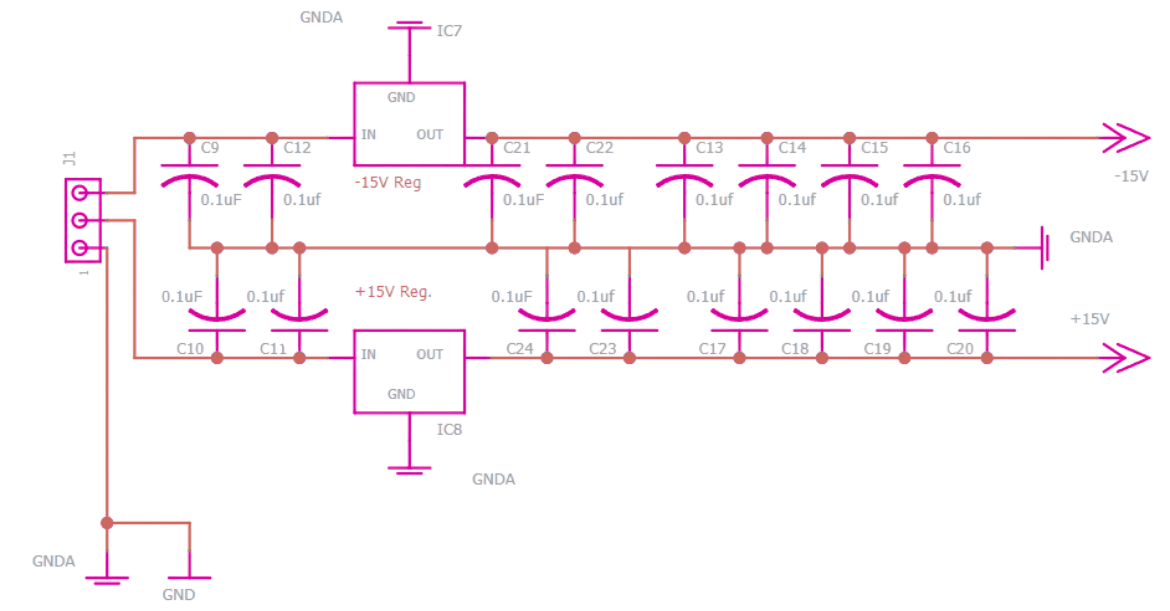
\includegraphics[width=0.7\textwidth]{images/ps.png}
    \end{figure}

\subsection{Controlled negative power source (NCC):}\label{ncc}

The negative voltage control is the most important aspect of our circuit. Because the laser needs a precise negative voltage to function correctly, this setup is essential. The LM337 regulator enables us to continuously vary the voltage between -1.2 V and -37 V. To prevent fluctuations, we also employ an NPN transistor with a rectifier diode, as well as a potentiometer for precise tuning. Input and output capacitors are also included to reduce noise and stabilize the current. This system maintains a steady voltage for the laser, avoiding instabilities that might impair the quality of the produced beam."


\begin{figure}[ht!]
            \centering
            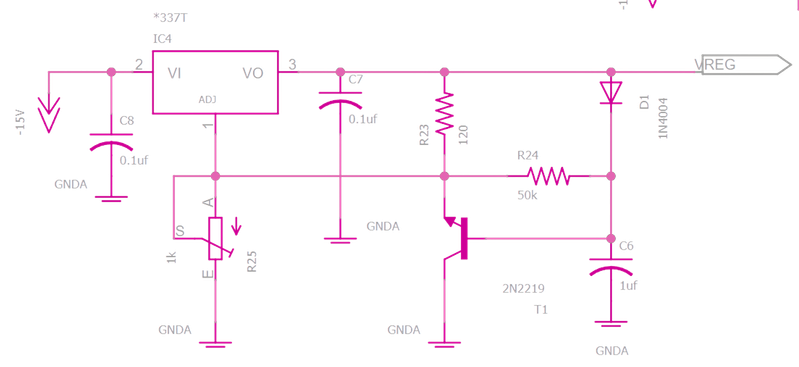
\includegraphics[width=0.7\textwidth]{images/ncc.png}
    \end{figure}

\subsection{Current control circuit (CC):}\label{cc}

Current management is another essential component of laser operation. We employ an LM399H-based circuit for this purpose, a high-stability, low-noise Zener diode utilized for accurate voltage references. Plus, we use an AD711N operational amplifier to compare the input voltage to a set reference, which helps to keep the laser's power supply current within ideal limits. The voltage-to-current conversion is regulated by a MOSFET, which serves as the control element, in order to avoid overloads and variations. This circuit helps us minimize signal noise, which is critical for achieving a high-quality, stable laser for spectroscopy.


    \begin{figure}[H]
            \centering
            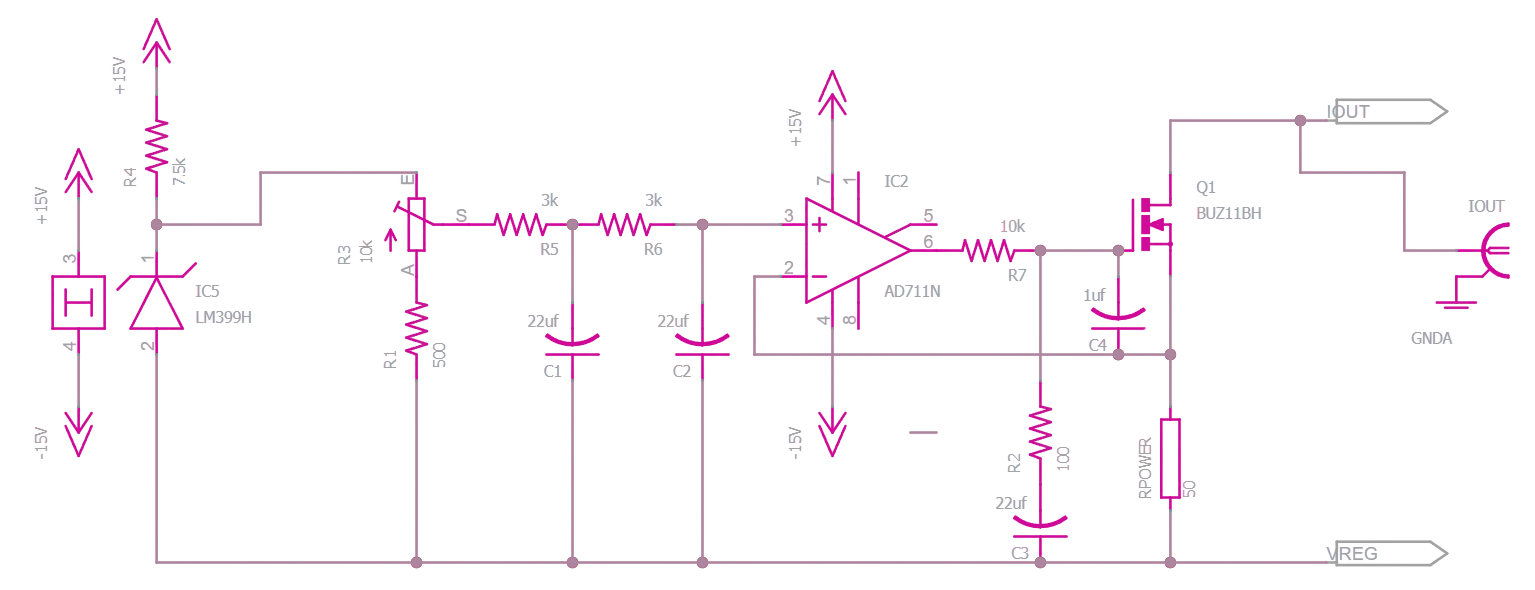
\includegraphics[width=0.7\textwidth]{images/cc.png}
    \end{figure}

\subsection{General control circuit (Switch):}\label{switch}

This circuit enables to on/off the laser and is the last checkup before damaging the laser diode.

    \begin{figure}[H]
            \centering
            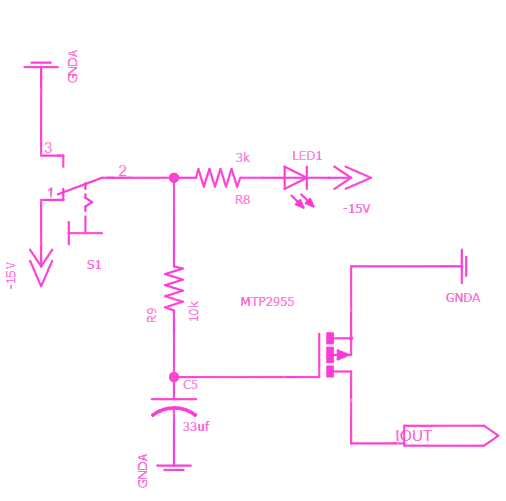
\includegraphics[width=0.4\textwidth]{images/switch.png}
    \end{figure}

\subsection{Modulation circuit (Mod):}\label{mod}
We implemented a modulation system that enables us to control the output power while simultaneously maintaining the beam frequency in order to enhance laser performance. Voltage modulation of the laser enables precise control over its intensity. Additionally, the laser's optical cavity is dynamically controlled by a piezoelectric element-based stabilization system. This system is especially helpful in spectroscopic applications, where it is essential to maintain beam coherence and avoid jumps that could compromise the precision of the measurement."

    \begin{figure}[H]
            \centering
            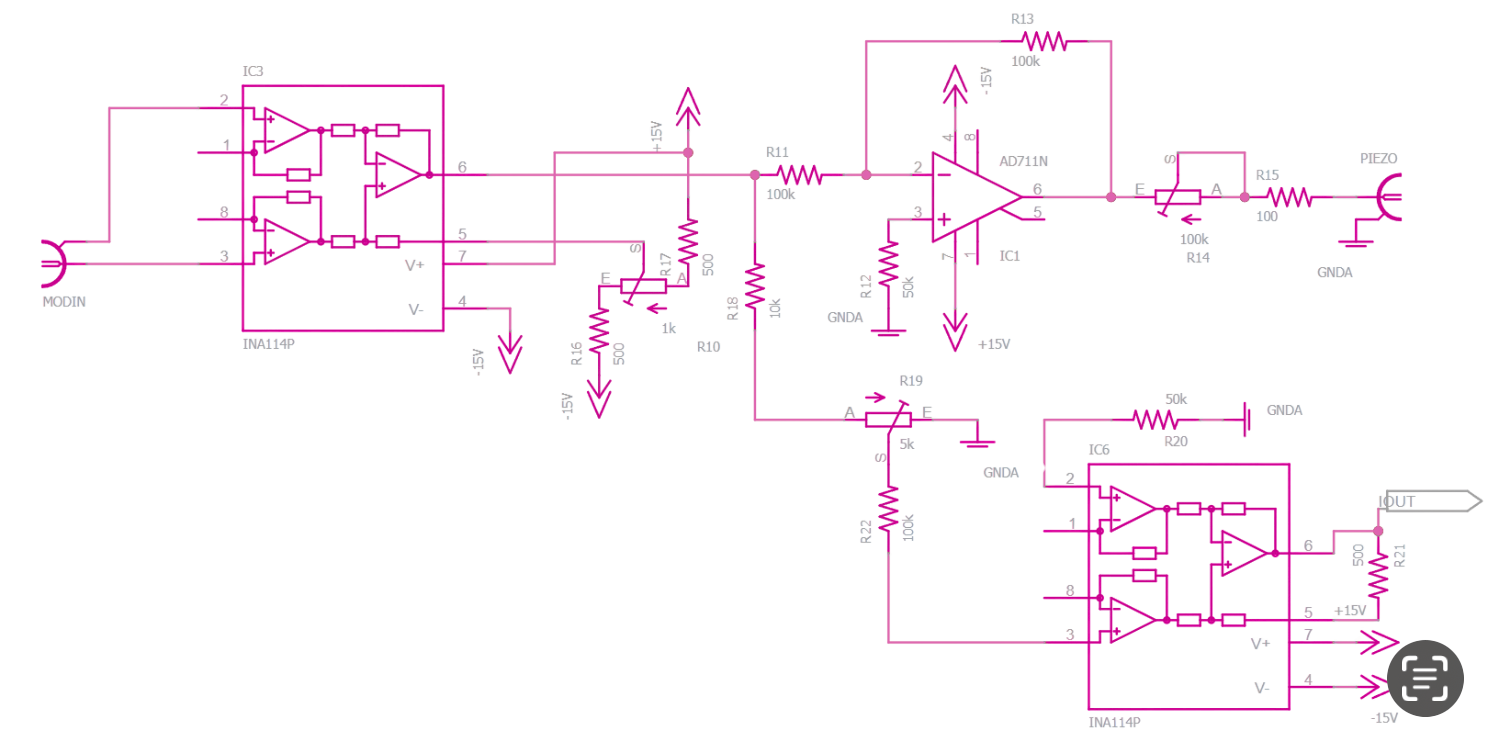
\includegraphics[width=0.7\textwidth]{images/mod}
    \end{figure}

\medskip
\newpage
\section{List of Components:}
% chktex-file 44
\begin{table}[ht]
\centering
    \begin{tabular}{|
    >{\columncolor[HTML]{ECF4FF}}l |l|l|l|}
    \hline
    \cellcolor[HTML]{F0A0D1}{\color[HTML]{000000} \textbf{Name}} &
    \cellcolor[HTML]{F0A0D1}{\color[HTML]{000000} \textbf{\#}} &
    \cellcolor[HTML]{F0A0D1}{\color[HTML]{000000} \textbf{Type}} &
    \cellcolor[HTML]{F0A0D1}\textbf{Circuit} \\ \hline
    \cellcolor[HTML]{ECF4FF}{\color[HTML]{000000} }         & 2 & 0.1 $\mu$ F       & PS              \\ \cline{2-4} 
    \cellcolor[HTML]{ECF4FF}{\color[HTML]{000000} }         & 3 & 1 $\mu$ F         & NCC, CC         \\ \cline{2-4} 
    \cellcolor[HTML]{ECF4FF}{\color[HTML]{000000} }         & 1 & 10 $\mu$ F        & NCC             \\ \cline{2-4} 
    \cellcolor[HTML]{ECF4FF}{\color[HTML]{000000} }         & 3 & 22 $\mu$ F        & CC              \\ \cline{2-4} 
    \cellcolor[HTML]{ECF4FF}{\color[HTML]{000000} }         & 1 & 33 $\mu$ F        & Switch          \\ \cline{2-4} 
    \multirow{-6}{*}{\cellcolor[HTML]{ECF4FF}{\color[HTML]{000000} Capacitor}} &
    1 &
    470 $\mu$ F &
    CC \\ \hline
    \cellcolor[HTML]{ECF4FF}                                & 3 & 100 $\Omega$      & NCC, CC, Mod    \\ \cline{2-4} 
    \cellcolor[HTML]{ECF4FF}                                & 4 & 500 $\Omega$      & CC, Mod         \\ \cline{2-4} 
    \cellcolor[HTML]{ECF4FF}                                & 3 & 3 K$\Omega$       & CC, Switch      \\ \cline{2-4} 
    \cellcolor[HTML]{ECF4FF}                                & 1 & 7,5 K$\Omega$     & CC              \\ \cline{2-4} 
    \cellcolor[HTML]{ECF4FF}                                & 3 & 10 K$\Omega$      & CC, Mod, Switch \\ \cline{2-4} 
    \cellcolor[HTML]{ECF4FF}                                & 3 & 50 K$\Omega$      & NCC, Mod        \\ \cline{2-4} 
    \multirow{-7}{*}{\cellcolor[HTML]{ECF4FF}Resistor}      & 3 & 100 K$\Omega$     & Mod             \\ \hline
    \cellcolor[HTML]{ECF4FF}                                & 2 & 1 K$\Omega$       & NCC, Mod        \\ \cline{2-4} 
    \cellcolor[HTML]{ECF4FF}                                & 1 & 5 K$\Omega$       & Mod             \\ \cline{2-4} 
    \cellcolor[HTML]{ECF4FF}                                & 1 & 10 K$\Omega$      & CC              \\ \cline{2-4} 
    \multirow{-4}{*}{\cellcolor[HTML]{ECF4FF}Potentiometer} & 1 & 100 K$\Omega$     & Mod             \\ \hline
    Rectifying diode                                        & 1 & 1N4007            & NCC             \\ \hline
    Laser diode                                             & 1 & L780P010         & Switch          \\ \hline
    Switch On/Off                                           & 1 & 100SP1T1B4M2QE    & Switch          \\ \hline
    Terminal Block                                          & 1 & MTA03\-100         & PS              \\ \hline
    \end{tabular}
\end{table}

\begin{table}[ht]
\centering
\resizebox{\textwidth}{!}{%
\begin{tabular}{|l|l|l|l|l|}
    \hline
    \rowcolor[HTML]{F0A0D1} 
    {\color[HTML]{000000} Name} &
    {\color[HTML]{000000} \#} &
    {\color[HTML]{000000} Type} &
    {\color[HTML]{000000} Circuit} &
    {\color[HTML]{000000} Datasheet} \\ \hline
    \cellcolor[HTML]{ECF4FF}{\color[HTML]{000000} } &
    1 &
    L7915ACV &
    PS &
    \url{https://www.alldatasheet.com/html-pdf/22637/STMICROELECTRONICS/L7915ACV/1622/1/L7915ACV.html} \\ \cline{2-5} 
    \multirow{-2}{*}{\cellcolor[HTML]{ECF4FF}{\color[HTML]{000000} Fixed voltage regulators}} &
    1 &
    L7815CV &
    PS &
    \url{https://www.alldatasheet.com/html-pdf/22641/STMICROELECTRONICS/L7815CV/1621/1/L7815CV.html} \\ \hline
    \cellcolor[HTML]{ECF4FF} &
    1 &
    LM337 &
    NCC &
    \url{https://www.alldatasheet.com/html-pdf/11667/ONSEMI/LM337/179/1/LM337.html} \\ \cline{2-5} 
    \multirow{-2}{*}{\cellcolor[HTML]{ECF4FF}Semiconductor} &
    1 &
    LM339 &
    CC &
    \url{https://www.alldatasheet.com/html-pdf/524807/STMICROELECTRONICS/LM339/1942/1/LM339.html} \\ \hline
    \cellcolor[HTML]{ECF4FF}NPN Transistor &
    1 &
    2N2219 &
    NCC &
    \url{https://www.alldatasheet.com/html-pdf/15066/PHILIPS/2N2219/245/1/2N2219.html} \\ \hline
    \cellcolor[HTML]{ECF4FF}Amplifier &
    2 &
    AD711N &
    CC, Mod &
    \url{https://www.alldatasheet.com/html-pdf/48159/AD/AD711/19/1/AD711.html} \\ \hline
    \cellcolor[HTML]{ECF4FF} &
    1 &
    n-channel BUZ11 &
    CC &
    \url{https://www.alldatasheet.com/html-pdf/22129/STMICROELECTRONICS/BUZ11/1619/1/BUZ11.html} \\ \cline{2-5} 
    \multirow{-2}{*}{\cellcolor[HTML]{ECF4FF}MOSFET} &
    1 &
    p-channel MTP2955 &
    Switch &
    \url{https://www.alldatasheet.com/html-pdf/5497/MOTOROLA/MTP2955/258/1/MTP2955.html} \\ \hline
    \cellcolor[HTML]{ECF4FF}R-power 50 &
    1 &
    IRF9530NS &
    CC &
    \url{https://www.alldatasheet.com/html-pdf/68327/IRF/IRF9530NS/48/1/IRF9530NS.html} \\ \hline
    \cellcolor[HTML]{ECF4FF}Instrumentation Amplifier &
    2 &
    INA114 &
    Mod &
    \url{https://www.alldatasheet.com/html-pdf/847617/TI1/INA114/53/1/INA114.html} \\ \hline
\end{tabular}
    }
\end{table}
\vfill

\begin{center}
    \begin{tikzpicture}
        \bee[cocktail,think={\small\color{black}\centering Thanks!}, bubblecolour=gray!30!white
]      
   \end{tikzpicture}
\end{center}


\end{document}
